\documentclass[a4paper, 10pt, twoside, notitlepage]{report}
% idioma
\usepackage[spanish]{babel}
\usepackage[utf8x]{inputenc}
% graficos
\usepackage[pdftex]{graphicx}
\usepackage{wrapfig}

%\usepackage{listings}
%\lstset{language=C,basicstyle=\small}

%\usepackage{epic,eepic}
% estilo
\usepackage[footnotesize]{caption}
\usepackage[outer=2cm,inner=4cm,top=2cm,bottom=2cm]{geometry}
\usepackage{fancyhdr}

\usepackage{color,hyperref}
\usepackage{enumerate}

\definecolor{black}{rgb}{0.0,0.0,0.0}
\definecolor{darkblue}{rgb}{0.0,0.0,0.3}

\hypersetup{colorlinks,breaklinks,
            linkcolor=black,urlcolor=darkblue,
            anchorcolor=darkblue,citecolor=darkblue}
            
\usepackage{blindtext}
\usepackage{listings}
% matematica
\usepackage{amsmath} 
\usepackage{amsfonts} 
\usepackage{amssymb}
\usepackage{enumitem}



 \title{U.B.A. - Facultad de Ingeniería\\\vspace{0.25cm} 66.20 Organización de Computadoras\\Guía de estudio}
  \author{Práctica jueves}
 \date{1° Cuatrimestre 2019}


\definecolor{mymauve}{rgb}{0.58,0,0.82}
\definecolor{mygreen}{rgb}{0,0.6,0}

\date{}

\begin{document}

\lstset{%
  basicstyle=\small\ttfamily,
  breaklines=true,
  tabsize=2,
  language=C,
  extendedchars=true
}

\lstdefinestyle{6620C}{
  identifierstyle=\color{blue},
  commentstyle=\color{mygreen},
  keywordstyle=\bfseries\color{mymauve},
  frame=single,
  breaklines=true
%  stringstyle=\color{purple}
}


\maketitle
\thispagestyle{empty}   % quita el número en la primer página

 \newpage
%\begin{abstract}

%\end{abstract}

 \tableofcontents
% 
 \newpage
% 

\pagestyle{fancy}
\fancyhead{}
\fancyfoot{}
\renewcommand{\sectionmark}[1]{\markright{\thesection\ #1}}
\renewcommand{\headrulewidth}{0.4pt}
\renewcommand{\chaptername}{Unidad}
%\renewcommand{\footrulewidth}{0.4pt}
\fancyhead[LE]{\nouppercase \rightmark}
\fancyhead[RE, LO]{\bf \thepage}
\fancyhead[RO]{\nouppercase \rightmark}
\fancyfoot[C]{ }
\maketitle
%genera el indice - compilar dos veces
\setcounter{page}{1}
% \tableofcontents
% \newpage

\parskip 7.2pt
\chapter*{Prólogo}
\addcontentsline{toc}{chapter}{Prólogo}
Durante varios cuatrimestres estuvo el interrogante si la deserción temprana y baja concurrencia no se debía a no contar con una guía fija y actualizada de ejercicios que ordene y estructure el curso.

La intención de este apunte es guiar al alumno a atravesar los temas de la materia con un breve resumen que sirve como introducción para luego si, atacar la bibliografía y poder resolver los ejercicios propuestos al final de cada capitulo. 

De ninguna manera se buscó que este apunte actúe como reemplazo de la basta bibliografía ni, menos como una traducción por más somera que sea, si bien muchas veces nos preguntamos que tanta incidencia traía esta barrera idiomática que extiende el material que utilizamos. Esperamos que sirva como motivación a los alumnos y que sirva como herramienta facilitadora para enfrentar esta materia.

\newcommand{\SU}{\textit{Speed Up }}
\newcommand*{\threeemdash}{\rule[0.5ex]{3em}{0.55pt}}
\section{Principios fundamentales}

\subsection{Ejercicio resuelto: [1.2 $3^{ed}$ CAAQA]}
Se considera realizar una mejora a una máquina agregando hardware vectorial. Cuando un cálculo de modo vectorial se ejecuta en este hardware, este se realiza 10 veces más rápido que en modo de ejecución normal. Llamamos al porcentaje de tiempo que se puede utilizar este modo vectorial como porcentaje de vectorización.


Antes de resolver el ejercicio, planteamos el escenario mediante un diagrama:

%TODO Usar un include
\tikzset{every picture/.style={line width=0.75pt}} %set default line width to 0.75pt

\begin{tikzpicture}[x=0.75pt,y=0.75pt,yscale=-1,xscale=1]
%uncomment if require: \path (0,300); %set diagram left start at 0, and has height of 300

%Shape: Rectangle [id:dp41842097652442645]
\draw   (39.5,21) -- (305.5,21) -- (305.5,61) -- (39.5,61) -- cycle ;
%Shape: Rectangle [id:dp8871764374832227]
\draw   (40.5,129) -- (304.5,129) -- (304.5,171) -- (40.5,171) -- cycle ;
%Shape: Rectangle [id:dp9269566177848496]
\draw   (305.5,21) -- (623.5,21) -- (623.5,61) -- (305.5,61) -- cycle ;
%Shape: Rectangle [id:dp3092576452949021]
\draw   (304.5,129) -- (380.5,129) -- (380.5,171) -- (304.5,171) -- cycle ;
%Straight Lines [id:da06697919884510961]
\draw  [dash pattern={on 0.84pt off 2.51pt}]  (305.5,61) -- (304.5,129) ;


%Straight Lines [id:da4571003142911374]
\draw  [dash pattern={on 0.84pt off 2.51pt}]  (623.5,61) -- (380.5,129) ;

% Text Node
\draw (21,41) node  [align=left] {$\displaystyle T_{O}$};
% Text Node
\draw (19,147) node  [align=left] {$\displaystyle T_{N}$};
% Text Node
\draw (424,42) node  [align=left] {$\displaystyle T_{M}$};
% Text Node
\draw (341.5,150) node  [align=left] {$\displaystyle T'_{M}$};
% Text Node
\draw (120,145) node  [align=left] {$ $};
% Text Node
\draw (151.5,150) node  [align=left] {$\displaystyle T'_{nm}$};
% Text Node
\draw (150.5,41) node  [align=left] {$\displaystyle T_{nm}$};

\end{tikzpicture}

\begin{enumerate}
 \item Realizar un gráfico que represente el \SU en función del como porcentaje de vectorización. Nombrar al \textit{eje y} como \SU Global ($SU_g$) y al \textit{eje x} como Porcentaje de Vectorización.

 Partiendo de la Ley de Amdahl, así como los datos del enunciado, tenemos que $$ SU_g = \frac{1}{(1-f) + \frac{f}{10}} = \frac{1}{1 - 0,9 \times f}$$
 Sabemos también que $ f \in [0, 1] $. Podemos calcular el valor de \SU en los extremos:
 \begin{itemize}
 \item Si no es posible aplicar la mejora, $f = 0 \implies SU_g = 1$
 \item Si la mejora es aplicable a todo el tiempo de ejecución, $ f = 1 \implies SU_g = SU_L = 10 $
 \end{itemize}

 \includegraphics[scale=0.5]{gfx/amdahl_resuelto_1.png}
 
 \threeemdash

 \item ¿Qué porcentaje de vectorización en necesaria para alcanzar un \SU global de 2?

 Utilizando la ley de Amdahl podemos despejar $f$

 $$ 2 = \frac{1}{1 - 0,9 \times f}$$
 $$ f  = \frac{5}{9} $$
 
 \threeemdash
 \item ¿Qué porcentaje de tiempo se emplea en modo vectorización cuando se alcanza un \SU global de 2?

 Es importante entender que esta pregunta no es igual a la anterior. El escenario para este punto nos plantea en el momento en el que 
 la optimización ya se encuentra en ejecución.

 Partiendo de la definición de Speed Up, tenemos que 

 $$ SU_g = \frac{T_O}{T_N} = 2 \implies f = \frac{5}{9} $$

 $$ SU_L = \frac{T_m}{T'_m} = 10,\quad siendo \quad T_m = T_O \times f = \frac{5}{9}T_O $$

 También es importante notar que $ T'_{nm} = T_{nm} = \frac{4}{9} \times T_O $, ya que el tiempo de ejecución de la parte del 
 programa en la que no se aplica ninguna optimización no cambia.
 
 El ejercicio nos pide calcular $ f' = \sfrac{T'_m}{T_N} $. Se puede determinar que
 
 $$ T'_m =  \sfrac{T_m}{10} $$ 
 $$ T_N = T'_{m} + T'_{nm} $$
 $$ T_{nm} = T'_{nm} $$ 
 
 $$ f' = \frac{\frac{5}{90}}{\frac{5}{90} + \frac{4}{9}} $$
 
 \threeemdash
 \item ¿Qué porcentaje de vectorización es necesaria para alcanzar la mitad del máximo \SU posible al usar el modo de vectorización?

 A partir de la Ley de Amdahl y el análisis realizado en el primer punto sabemos qué $SU_{max} = 10$, por lo que solo resta resolver

 $$ \frac{1}{5} = 1 - 0,9 \times f $$
 $$ f = \frac{8}{9} $$ 
 
 \threeemdash
 \item Ahora suponga que se realizó una medición y se determinó que el porcentaje de vectorización para ciertos programas es del 70\%. El grupo de diseño de hardware dice que pueden duplicar el \SU del hardware de vectorización pero con una inversión significante en lo que respecta. Entonces nos preguntamos si el equipo de compiladores podrían incrementar el uso del modo vectorizado (relativo al uso actual) para lograr la misma performance obtenida al aumentar al doble el \SU por hardware. ¿Qué inversión recomendaría?  

\end{enumerate}


\subsection{}
Demostrar que 

						 $$ SU = \frac {1} {(1-f) + \frac {f}{SU_L}} $$


Donde $f$ es la fracción de tiempo a mejorar, y $SU_L$ es la mejora local.

\subsection{}

Un procesador de 300 Mhz ejecuta un programa que presenta los siguientes tipos de instrucciones:

\begin{table}[h!]
\begin{tabular}{|l|c|c|}
\hline
 Tipo de instrucción & Frecuencia (\%)  &  Ciclos  \\ \hline
 Aritmético-Lógica & 40  &  1  \\ \hline
 Carga & 20 & 1 \\ \hline
 Almacenamiento & 10  & 2  \\ \hline
 Saltos & 20  & 3 \\ \hline
 Punto Flotante & 10 & 5  \\ \hline
\end{tabular}
\end{table}

\begin{enumerate}[label=\alph*)]
 \item Calcular las tasas de CPI y MIPS, para el programa completo.
 \item Suponga que una optimización elimina un 30 \% de las instrucciones aritmético-lógicas (o sea, 12 \% del total de instrucciones A-L), 30 \% de instrucciones load y 20 \% de punto flotante. ¿Cuál es el speedup alcanzado?
 \item Recalcular las tasas de CPI y MIPS para el programa completo. Explicar las diferencias respecto al punto (a).
\end{enumerate}

\subsection{}
Se proponen 3 mejoras para una nueva arquitectura con los siguientes Speedups:
\begin{itemize}
\item Speedup1 = 30
\item Speedup2 = 20
\item Speedup3 = 10
\end{itemize}

Sólo una mejora es aplicable en cada momento (no se pueden solapar).

\begin{enumerate}[label=\alph*)]
 \item Si las mejoras 1 y 2 se pueden usar un 30 \% del tiempo, ¿qué fracción del tiempo se debe usar la mejora 3 para lograr un speedup global de 10?
 \item Asumir que la distribución del uso de las mejoras es del 30 \%, 30 \% y 20 para las mejoras 1, 2 y 3 respectivamente. Asumir que las 3 mejoras están en uso. ¿Qué fracción del tiempo mejorado no tiene una mejora en uso?
 \item Asumir que para un benchmark la fracción del uso de las mejoras es del 15 \% para 1 y 2 y del 70 \% para la mejora 3. Se quiere maximizar la performance. Si sólo una mejora puede ser aplicada, ¿cuál debería ser elegida? Si 2 mejoras pueden ser aplicadas, ¿cuales deberían ser elegidas?
\end{enumerate}

\subsection{}
Se dispone de un benchmark que contiene $195,578$ instrucciones de punto flotante.
	
Dicho Benchmark fue ejecutado en un procesador embebido luego de haber sido compilado con las optimizaciones activadas. El procesador embebido está basado en un procesador RISC que incluye unidades de punto flotante, pero el procesador embebido no dispone de ellas por distintas razones. El compilador permite calcular las operaciones de punto flotante mediante unidades punto flotante o mediante rutinas de software, dependiendo en las opciones utilizadas.
	
El benchmark se ejecutó en $1,08$ segundos en el procesador RISC, mientras que tomó $13.6$ segundos en la versión embebida. Asumir que el CPI del procesador RISC es $10$, mientras que el CPI del procesador embebido es $6$.
	
\begin{enumerate}[label=\alph*)]
\item Para ambos procesadores, ¿cuántas instrucciones fueron ejecutadas?
\item Para ambos procesadores, ¿cuál es el valor de la tasa de MIPS?
\item En promedio, ¿cuántas instrucciones enteras son necesarias para ejecutar una operación de punto flotante en software?
\end{enumerate}
	
Responder considerando que el benchmark puede estar conformado por 
	
\begin{itemize}
    \item Un $100\%$ de instrucciones de punto flotante.
    \item Instrucciones de punto flotante y enteras.
\end{itemize}


\subsection{[1.3 $3^{ed}$ CAAQA]}
Se realiza una mejora a una computadora a un dado modo de ejecución por un factor de 10. Esta mejora es utilizada el 50\% del tiempo, medido como un porcentaje del tiempo de ejecución cuando la mejora está siendo utilizada. Recordar que no se puede aplicar directamente este 50\% en la Ley de Amdahl para para calcular el speedup.

\begin{enumerate}
 \item ¿Cuál es el speedup global que se alcanza con esta mejora?
 \item ¿Qué porcentaje del tiempo original es empleada esta mejora?
\end{enumerate}


\subsection{[1.6 $3^{ed}$ CAAQA]}
Un benchmark muy conocido para enteros es Dhrystone. La computadora A realiza D A ejecuciones del benchmark por segundo y realiza millones de instrucciones por segundo (MIPS A). En la computadora B se ejecuta el mismo benchmark obteniendo sus propias métricas.

\begin{enumerate}
 \item ¿Cuál es el problema en calcular la tasa de MIPS de la computadora B como $MIPS_B = MIPS_A \times (D_B / D_A )$?
\end{enumerate}



\subsection{[1.17 $3^{ed}$ CAAQA]}
Una empresa tiene un benchmark que es considerado representativo para sus aplicaciones típicas. Se está considerando un procesador embebido para realizar las tareas pero no cuenta con una unidad de punto flotante y se deben emular por una secuencia de instrucciones de enteros. Este procesador tiene una tasa de 120 MIPS en el benchmark.

Un vendedor ofrece un coprocesador para mejorar la performance. Este coprocesador ejecuta cada instrucción de punto flotante por hardware. Cuando se combina el procesador y el coprocesador resulta una tasa de MIPS de 80 en el mismo benchmark.

Sea:

\begin{itemize}
 \item I: Número de instrucciones de enteros ejecutadas en el benchmark.
 \item F: Número de instrucciones de punto flotante ejecutadas en el benchmark.
 \item Y: Número de instrucciones de entero para emular las instrucciones de punto flotante.
 \item W: Tiempo de ejecución del benchmark en el procesador solo.
 \item B: Tiempo de ejecución del benchmark en la combinación procesador/coprocesador.
\end{itemize}

\begin{enumerate}
 \item Escribir una expresión para calcular la tasa de MIPS en cada configuración utilizando los símbolos anteriores.
 \item Para la configuración sin coprocesador, se obtuvo $F = 8 \times 10^6$, $Y = 50$ y $W = 4$ segundos. Determinar I.
 \item ¿Cuál es el valor de B?
 \item ¿Cuál es la tasa de MFLOPS para el sistema con coprocesador?
 \item Un colega quiere comprar el coprocesador a pesar que tiene una tasa de MIPS inferior cuando se lo utiliza en comparación con el procesador sólo. ¿Tiene razón? Justificar la respuesta.
\end{enumerate}



% \newcommand{\SU}{\textit{Speed Up }}
\newcommand*{\threeemdash}{\rule[0.5ex]{3em}{0.55pt}}
\section{Principios fundamentales}

\subsection{Ejercicio resuelto: [1.2 $3^{ed}$ CAAQA]}
Se considera realizar una mejora a una máquina agregando hardware vectorial. Cuando un cálculo de modo vectorial se ejecuta en este hardware, este se realiza 10 veces más rápido que en modo de ejecución normal. Llamamos al porcentaje de tiempo que se puede utilizar este modo vectorial como porcentaje de vectorización.


Antes de resolver el ejercicio, planteamos el escenario mediante un diagrama:

%TODO Usar un include
\tikzset{every picture/.style={line width=0.75pt}} %set default line width to 0.75pt

\begin{tikzpicture}[x=0.75pt,y=0.75pt,yscale=-1,xscale=1]
%uncomment if require: \path (0,300); %set diagram left start at 0, and has height of 300

%Shape: Rectangle [id:dp41842097652442645]
\draw   (39.5,21) -- (305.5,21) -- (305.5,61) -- (39.5,61) -- cycle ;
%Shape: Rectangle [id:dp8871764374832227]
\draw   (40.5,129) -- (304.5,129) -- (304.5,171) -- (40.5,171) -- cycle ;
%Shape: Rectangle [id:dp9269566177848496]
\draw   (305.5,21) -- (623.5,21) -- (623.5,61) -- (305.5,61) -- cycle ;
%Shape: Rectangle [id:dp3092576452949021]
\draw   (304.5,129) -- (380.5,129) -- (380.5,171) -- (304.5,171) -- cycle ;
%Straight Lines [id:da06697919884510961]
\draw  [dash pattern={on 0.84pt off 2.51pt}]  (305.5,61) -- (304.5,129) ;


%Straight Lines [id:da4571003142911374]
\draw  [dash pattern={on 0.84pt off 2.51pt}]  (623.5,61) -- (380.5,129) ;

% Text Node
\draw (21,41) node  [align=left] {$\displaystyle T_{O}$};
% Text Node
\draw (19,147) node  [align=left] {$\displaystyle T_{N}$};
% Text Node
\draw (424,42) node  [align=left] {$\displaystyle T_{M}$};
% Text Node
\draw (341.5,150) node  [align=left] {$\displaystyle T'_{M}$};
% Text Node
\draw (120,145) node  [align=left] {$ $};
% Text Node
\draw (151.5,150) node  [align=left] {$\displaystyle T'_{nm}$};
% Text Node
\draw (150.5,41) node  [align=left] {$\displaystyle T_{nm}$};

\end{tikzpicture}

\begin{enumerate}
 \item Realizar un gráfico que represente el \SU en función del como porcentaje de vectorización. Nombrar al \textit{eje y} como \SU Global ($SU_g$) y al \textit{eje x} como Porcentaje de Vectorización.

 Partiendo de la Ley de Amdahl, así como los datos del enunciado, tenemos que $$ SU_g = \frac{1}{(1-f) + \frac{f}{10}} = \frac{1}{1 - 0,9 \times f}$$
 Sabemos también que $ f \in [0, 1] $. Podemos calcular el valor de \SU en los extremos:
 \begin{itemize}
 \item Si no es posible aplicar la mejora, $f = 0 \implies SU_g = 1$
 \item Si la mejora es aplicable a todo el tiempo de ejecución, $ f = 1 \implies SU_g = SU_L = 10 $
 \end{itemize}

 \includegraphics[scale=0.5]{gfx/amdahl_resuelto_1.png}
 
 \threeemdash

 \item ¿Qué porcentaje de vectorización en necesaria para alcanzar un \SU global de 2?

 Utilizando la ley de Amdahl podemos despejar $f$

 $$ 2 = \frac{1}{1 - 0,9 \times f}$$
 $$ f  = \frac{5}{9} $$
 
 \threeemdash
 \item ¿Qué porcentaje de tiempo se emplea en modo vectorización cuando se alcanza un \SU global de 2?

 Es importante entender que esta pregunta no es igual a la anterior. El escenario para este punto nos plantea en el momento en el que 
 la optimización ya se encuentra en ejecución.

 Partiendo de la definición de Speed Up, tenemos que 

 $$ SU_g = \frac{T_O}{T_N} = 2 \implies f = \frac{5}{9} $$

 $$ SU_L = \frac{T_m}{T'_m} = 10,\quad siendo \quad T_m = T_O \times f = \frac{5}{9}T_O $$

 También es importante notar que $ T'_{nm} = T_{nm} = \frac{4}{9} \times T_O $, ya que el tiempo de ejecución de la parte del 
 programa en la que no se aplica ninguna optimización no cambia.
 
 El ejercicio nos pide calcular $ f' = \sfrac{T'_m}{T_N} $. Se puede determinar que
 
 $$ T'_m =  \sfrac{T_m}{10} $$ 
 $$ T_N = T'_{m} + T'_{nm} $$
 $$ T_{nm} = T'_{nm} $$ 
 
 $$ f' = \frac{\frac{5}{90}}{\frac{5}{90} + \frac{4}{9}} $$
 
 \threeemdash
 \item ¿Qué porcentaje de vectorización es necesaria para alcanzar la mitad del máximo \SU posible al usar el modo de vectorización?

 A partir de la Ley de Amdahl y el análisis realizado en el primer punto sabemos qué $SU_{max} = 10$, por lo que solo resta resolver

 $$ \frac{1}{5} = 1 - 0,9 \times f $$
 $$ f = \frac{8}{9} $$ 
 
 \threeemdash
 \item Ahora suponga que se realizó una medición y se determinó que el porcentaje de vectorización para ciertos programas es del 70\%. El grupo de diseño de hardware dice que pueden duplicar el \SU del hardware de vectorización pero con una inversión significante en lo que respecta. Entonces nos preguntamos si el equipo de compiladores podrían incrementar el uso del modo vectorizado (relativo al uso actual) para lograr la misma performance obtenida al aumentar al doble el \SU por hardware. ¿Qué inversión recomendaría?  

\end{enumerate}


\subsection{}
Demostrar que 

						 $$ SU = \frac {1} {(1-f) + \frac {f}{SU_L}} $$


Donde $f$ es la fracción de tiempo a mejorar, y $SU_L$ es la mejora local.

\subsection{}

Un procesador de 300 Mhz ejecuta un programa que presenta los siguientes tipos de instrucciones:

\begin{table}[h!]
\begin{tabular}{|l|c|c|}
\hline
 Tipo de instrucción & Frecuencia (\%)  &  Ciclos  \\ \hline
 Aritmético-Lógica & 40  &  1  \\ \hline
 Carga & 20 & 1 \\ \hline
 Almacenamiento & 10  & 2  \\ \hline
 Saltos & 20  & 3 \\ \hline
 Punto Flotante & 10 & 5  \\ \hline
\end{tabular}
\end{table}

\begin{enumerate}[label=\alph*)]
 \item Calcular las tasas de CPI y MIPS, para el programa completo.
 \item Suponga que una optimización elimina un 30 \% de las instrucciones aritmético-lógicas (o sea, 12 \% del total de instrucciones A-L), 30 \% de instrucciones load y 20 \% de punto flotante. ¿Cuál es el speedup alcanzado?
 \item Recalcular las tasas de CPI y MIPS para el programa completo. Explicar las diferencias respecto al punto (a).
\end{enumerate}

\subsection{}
Se proponen 3 mejoras para una nueva arquitectura con los siguientes Speedups:
\begin{itemize}
\item Speedup1 = 30
\item Speedup2 = 20
\item Speedup3 = 10
\end{itemize}

Sólo una mejora es aplicable en cada momento (no se pueden solapar).

\begin{enumerate}[label=\alph*)]
 \item Si las mejoras 1 y 2 se pueden usar un 30 \% del tiempo, ¿qué fracción del tiempo se debe usar la mejora 3 para lograr un speedup global de 10?
 \item Asumir que la distribución del uso de las mejoras es del 30 \%, 30 \% y 20 para las mejoras 1, 2 y 3 respectivamente. Asumir que las 3 mejoras están en uso. ¿Qué fracción del tiempo mejorado no tiene una mejora en uso?
 \item Asumir que para un benchmark la fracción del uso de las mejoras es del 15 \% para 1 y 2 y del 70 \% para la mejora 3. Se quiere maximizar la performance. Si sólo una mejora puede ser aplicada, ¿cuál debería ser elegida? Si 2 mejoras pueden ser aplicadas, ¿cuales deberían ser elegidas?
\end{enumerate}

\subsection{}
Se dispone de un benchmark que contiene $195,578$ instrucciones de punto flotante.
	
Dicho Benchmark fue ejecutado en un procesador embebido luego de haber sido compilado con las optimizaciones activadas. El procesador embebido está basado en un procesador RISC que incluye unidades de punto flotante, pero el procesador embebido no dispone de ellas por distintas razones. El compilador permite calcular las operaciones de punto flotante mediante unidades punto flotante o mediante rutinas de software, dependiendo en las opciones utilizadas.
	
El benchmark se ejecutó en $1,08$ segundos en el procesador RISC, mientras que tomó $13.6$ segundos en la versión embebida. Asumir que el CPI del procesador RISC es $10$, mientras que el CPI del procesador embebido es $6$.
	
\begin{enumerate}[label=\alph*)]
\item Para ambos procesadores, ¿cuántas instrucciones fueron ejecutadas?
\item Para ambos procesadores, ¿cuál es el valor de la tasa de MIPS?
\item En promedio, ¿cuántas instrucciones enteras son necesarias para ejecutar una operación de punto flotante en software?
\end{enumerate}
	
Responder considerando que el benchmark puede estar conformado por 
	
\begin{itemize}
    \item Un $100\%$ de instrucciones de punto flotante.
    \item Instrucciones de punto flotante y enteras.
\end{itemize}


\subsection{[1.3 $3^{ed}$ CAAQA]}
Se realiza una mejora a una computadora a un dado modo de ejecución por un factor de 10. Esta mejora es utilizada el 50\% del tiempo, medido como un porcentaje del tiempo de ejecución cuando la mejora está siendo utilizada. Recordar que no se puede aplicar directamente este 50\% en la Ley de Amdahl para para calcular el speedup.

\begin{enumerate}
 \item ¿Cuál es el speedup global que se alcanza con esta mejora?
 \item ¿Qué porcentaje del tiempo original es empleada esta mejora?
\end{enumerate}


\subsection{[1.6 $3^{ed}$ CAAQA]}
Un benchmark muy conocido para enteros es Dhrystone. La computadora A realiza D A ejecuciones del benchmark por segundo y realiza millones de instrucciones por segundo (MIPS A). En la computadora B se ejecuta el mismo benchmark obteniendo sus propias métricas.

\begin{enumerate}
 \item ¿Cuál es el problema en calcular la tasa de MIPS de la computadora B como $MIPS_B = MIPS_A \times (D_B / D_A )$?
\end{enumerate}



\subsection{[1.17 $3^{ed}$ CAAQA]}
Una empresa tiene un benchmark que es considerado representativo para sus aplicaciones típicas. Se está considerando un procesador embebido para realizar las tareas pero no cuenta con una unidad de punto flotante y se deben emular por una secuencia de instrucciones de enteros. Este procesador tiene una tasa de 120 MIPS en el benchmark.

Un vendedor ofrece un coprocesador para mejorar la performance. Este coprocesador ejecuta cada instrucción de punto flotante por hardware. Cuando se combina el procesador y el coprocesador resulta una tasa de MIPS de 80 en el mismo benchmark.

Sea:

\begin{itemize}
 \item I: Número de instrucciones de enteros ejecutadas en el benchmark.
 \item F: Número de instrucciones de punto flotante ejecutadas en el benchmark.
 \item Y: Número de instrucciones de entero para emular las instrucciones de punto flotante.
 \item W: Tiempo de ejecución del benchmark en el procesador solo.
 \item B: Tiempo de ejecución del benchmark en la combinación procesador/coprocesador.
\end{itemize}

\begin{enumerate}
 \item Escribir una expresión para calcular la tasa de MIPS en cada configuración utilizando los símbolos anteriores.
 \item Para la configuración sin coprocesador, se obtuvo $F = 8 \times 10^6$, $Y = 50$ y $W = 4$ segundos. Determinar I.
 \item ¿Cuál es el valor de B?
 \item ¿Cuál es la tasa de MFLOPS para el sistema con coprocesador?
 \item Un colega quiere comprar el coprocesador a pesar que tiene una tasa de MIPS inferior cuando se lo utiliza en comparación con el procesador sólo. ¿Tiene razón? Justificar la respuesta.
\end{enumerate}



\documentclass{beamer}

\usepackage[utf8]{inputenc}
\usetheme{default}

\usepackage{listings}
\lstset{
basicstyle=\small\ttfamily,
columns=flexible,
breaklines=true
}

\usepackage{epstopdf}
\usepackage{multicol}
\usepackage{caption}

\makeatletter
\DeclareMathSizes{\f@size}{10}{7}{7}
\makeatother

\title[66.20/86.37]{U.B.A. - Facultad de Ingeniería\\\vspace{0.25cm} 66.20/86.37 Organización de Computadoras
\\Arquitecturas}
\author{Práctica}
\date{2$^{do}$ cuatrimestre 2020}


\begin{document}
\begin{frame}
\titlepage % Print the title page as the first frame
\end{frame}

\begin{frame}
\frametitle{Clasificación de ISAs}
\begin{center}
 \includegraphics[scale=.45,keepaspectratio=true]{ISA.png}
\end{center}
\end{frame}

\begin{frame}
 \frametitle{Clasificación de ISAs}
 \begin{itemize}
  \item Modelo de pila: 
Los operandos están implícitamente en el tope del stack y el hardware debe evaluar la expresión en un solo orden y cargar un operando múltiples veces.
\item Modelo de acumulador: 
En una arquitectura de acumulador un operando está implícito en el acumulador.
\item Modelo de registros de propósito general: 
Aquí se tienen únicamente operandos explícitos, ya sea que estén ubicados en registros o en memoria.
\item Modelo de carga y almacenamiento: 
En este tipo de arquitectura, la memoria solo puede ser accedida a través de instrucciones de carga y almacenamiento (load/store). 
 \end{itemize}
\end{frame}


\begin{frame}
 \frametitle{Tipo de instrucciones en MIPS}
 \begin{itemize}
  \item Load / Store: únicas que acceden a memoria.
  \item Computational: realizadas en la ALU.
  \item Jump / Branch: saltos incondicionales y condicionales.
  \item Miscelaneas: Serialización de instrucciones, Excepciones (syscall), Moves condicionales, Prefetch, NOPs.
  \item Coprocessors y FPU.
 \end{itemize}
\end{frame}



\begin{frame}
 \frametitle{Endianess}
Todo el conjunto de instrucciones es direccionado por bytes y se provee acceso por bytes (8 bits), mitad de palabra (half words) (16 bits), por palabra (words) (32 bits).

\bigskip

Hay dos convenciones para ordenar los bytes en un objeto. \textbf{Little Endian} y \textbf{Big Endian}.
 \end{frame}
 
\begin{frame}
 \frametitle{Endianess}

El orden \textbf{Little Endian} coloca el byte cuya dirección "x . . . x000” en la posición menos significativa. Los bytes entonces son numerados:

  \begin{center}
 \includegraphics[scale=.7,keepaspectratio=true]{little_endian.png}
\end{center}


El orden \textbf{Big Endian} coloca el byte cuya dirección es “x . . . x000”  en la posición más significativa. Los bytes entonces son numerados:

\begin{center}
 \includegraphics[scale=.7,keepaspectratio=true]{big_endian.png}
\end{center}

 \end{frame}


\begin{frame}
 \frametitle{Alineación}
 En varias computadoras, los accesos a objetos más grandes que un byte deben estar alineados.
 \begin{itemize}
  \item Un objeto de tamaño s bytes en la dirección de bytes A está alineado si
    A mod s = 0.
  \item Esto se fuerza en muchas arquitecturas porque el hardware accede a
    memoria típicamente alineado a múltiplos de word o double-word.
 \end{itemize}
\bigskip
 ¿Qué puede ocurrir a nivel de accesos a memoria si se accede a datos no alineados y la arquitectura lo permite?
    
\end{frame}

\begin{frame}
 \frametitle{Modos de direccionamiento}
Se presentan varios modos de direccionamiento: 
\begin{multicols}{2}
\begin{itemize}
 \item Register
 \item Immediate
 \item Displacement
 \item Register indirect
 \item Indexed
 \item Direct or Absolute
 \item Memory indirect
 \item Autoincrement
 \item Autodecrement
 \item Scaled
 \end{itemize}
\end{multicols}

MIPS implementa 2 modos de direccionamiento: Immediate y Displacement, ambos con immediate de 16 bits.
    
Usando el registro 0 se consigue Absolute, y con displacement 0 se consigue Register indirect.
\end{frame}

\begin{frame}[fragile]
\frametitle{Modos de direccionamiento}

\begin{lstlisting}
    Immediate:		add	$t1, $t2, 10	
    Displacement:	lw	$t1, 30($t2)
    Absolute:		sb	$t1, 40($0)
    Indirect:		sw	$t1, 0($t2)
\end{lstlisting}
\end{frame}


\begin{frame}
 \frametitle{Encoding MIPS} 
 Hay 3 formatos de encoding posibles en MIPS
 \begin{itemize}
  \item I-type (Immediate)
  \item R-type (Register)
  \item J-type (Jump)
 \end{itemize}
\end{frame}

\begin{frame}
 \frametitle{Encoding MIPS} 
 
 \begin{center}
 \includegraphics[scale=.4,keepaspectratio=true]{tipos_instruccion.png}
\end{center}
 \end{frame}


\begin{frame}
 \frametitle{Encoding MIPS} 

 Viendo el detalle de las instrucciones J-type vemos que hay un offset de 26 bits left-shifted 2 bits, para formar los 28 lsb de la direccion destino del salto (las regiones de salto están alineadas a 256MB, y la región está determinada por los 4 msb de PC).
 
 \bigskip

 ¿Por qué se puede (y conviene) tomar los 26 bits como desplazados a la izquierda 2 bits?
\end{frame}

     
\end{document}

\section{Architecture Binary Interface}
Esta sección no pretende ser una descripción completa de la ABI presentada en \cite{abi}, sino un detalle de los puntos que se consideran confusos, más importantes o que varían respecto al documento mencionado.

Esta explicación se basa en \cite{abi} y en las observaciones realizadas sobre código assembly generado con GCC, con nivel de optimización 0 (−O0).

Por lo tanto, se recomienda primero leer la sección “Function Calling Sequence” de \cite{abi}, para luego aclarar y/o modificar con el contenido de este documento.

\subsection{Caller y Callee Saved Registers}
Los siguientes registros deben ser salvados por la función llamada si ésta los debe modificar:

\begin{itemize}
 \item ra, sp, fp (o s8), gp, s0...s7
 \item f20 a f30 (floating point)
\end{itemize}

El resto de los registros no se garantiza que su valor se preserve entre llamadas a funciones. Si la función caller necesita preservarlos, debe salvarlos ella en su stack frame.

\subsection{Stack Frame}
Cada función crea su Stack Frame siempre.

El Stack Frame se compone de areas de un tamaño múltiplo de 8 bytes, alineadas a 8 bytes.

Los registros en un area se almacenan de abajo hacia arriba, en orden según el número de registro.

Las areas son, en orden de aparición (de arriba hacia abajo en memoria):

\begin{itemize}
 \item General Register Save Area (obligatoria). Registros salvados:
 \begin{itemize}
  \item Siempre: fp, gp;
  \item Cuando la función es non-leaf: ra;
  \item Si es necesario: el resto de los general purpose callee-saved regs.
 \end{itemize}
\item Floating-Point Registers Save Area: f20 a f30 si es necesario (ver 3-15 de \cite{abi} para más detalle)
\item Local and Temporary Variables Area;
\item Argument Building Area.
\begin{itemize}
 \item Se crea cuando la función es non-leaf
 \item Al menos es de 16 bytes, aún cuando los argumentos del callee
requieren menos.
 \item Cuando los cuatro primeros argumentos son enteros o punteros,
se pasan en a0 a a3, y el resto se guarda en esta area a partir de
los primeros 16 bytes.
 \item Los argumentos pasados en a0 a a3 son almacenados en esta area
por el callee siempre.
\end{itemize}
\end{itemize}

\begin{table}[!h]
\begin{center}
\begin{tabular}{|c|}\hline
Saved Regs Area (*)\\\hline
Float Regs Area\\\hline
Local Area\\\hline
Arg Building Area
$\leq$ 16 bytes\\\hline
\end{tabular}
\caption{Layout genérico del stack frame. Las areas marcadas con (*) son obligatorias.}
\end{center}
\end{table}


Debugging: algunas reglas de creación de stack frame existen sólo para
garantizar que las herramientas de debugging (ej: gdb) puedan puedan
realizar un stack backtrace (es decir, algunas reglas pueden no seguirse y
el programa funcionará correctamente, pero no se garantiza un correcto
analisis post-mortem en caso de que el proceso termine de forma anormal).

\begin{table}[!h]
\begin{center}
\begin{tabular}{|c|}\hline
fp (\$30)\\\hline
gp (\$28)\\\hline
\end{tabular}
\caption{Ejemplo de Saved Regs Area mínima - función leaf.}
\end{center}
\end{table}


\begin{table}[!h]
\begin{center}
\begin{tabular}{|c|}\hline
alignment [4]\\\hline
ra (\$31)\\\hline
fp (\$30)\\\hline
gp (\$28)\\\hline
\end{tabular}
\caption{Ejemplo de Saved Regs Area mínima para una función non-leaf. También puede salvar el resto de los callee-saved registers.}
\end{center}
\end{table}

% \section{Arquitectura de Conjunto de Instrucciones (ISA)}
         \begin{center}
         \captionof{table}{\textit{Mix. de instrucciones}}\label{fig::232}
         \begin{tabular}{||l|c||}
         \hline
         Instrucción & Frecuencia \\\hline
         \textit{Load} & $26\%$ \\\hline
         \textit{Store} & $10\%$ \\\hline
         Aritméticas & $14\%$ \\\hline
         Comparaciones & $13\%$ \\\hline
         Saltos condicionales & $16\%$ \\\hline
         Saltos incondicionales & $1\%$ \\\hline
         \textit{Call / Return} & $2\%$ \\\hline
         Shift & $4\%$ \\\hline
         Logicas & $4\%$ \\\hline
         Misc. & $5\%$ \\\hline
         \end{tabular}
         \end{center}

\subsection{}
         %      \begin{small}
%            \begin{verbatim}                                   
%            Instruction     gap    gcc    gzip   mcf    perl   I. average
%            load           44.7%   35.5%  31.8%  33.2%  41.6%   37%
%            store          10.3%   13.2%  5.1%   4.3%   16.2%   10%
%            add             7.7%   11.2%  16.8%  7.2%   5.5%    10%
%            sub             1.7%   2.2%   5.1%   3.7%   2.5%    3%
%            mul             1.4%   0.1%                         0%
%            compare         2.8%   6.1%   6.6%   6.3%   3.8%    5%
%            cond branch     9.3%   12.1%  11.0%  17.5%  10.9%   12%
%            cond move       0.4%   0.6%   1.1%   0.1%   1.9%    1%
%            jump            0.8%   0.7%   0.8%   0.7%   1.7%    1%
%            call            1.6%   0.6%   0.4%   3.2%   1.1%    1%
%            return          1.6%   0.6%   0.4%   3.2%   1.1%    1%
%            shift           3.8%   1.1%   2.1%   1.1%   0.5%    2%
%            and             4.3%   4.6%   9.4%   0.2%   1.2%    4%
%            or              7.9%   8.5%   4.8%   17.6%  8.7%    9%
%            xor             1.8%   2.1%   4.4%   1.5%   2.8%    3%
%            other logical   0.1%   0.4%   0.1%   0.1%   0.3%    0%
%            load FP                                             0%
%            store FP                                            0%
%            add FP                                              0%
%            sub FP                                              0%
%            mul FP                                              0%
%            div FP                                              0%
%            mov reg-reg FP                                      0%
%            compare FP                                          0%
%            cond mov FP                                         0%
%            other FP                                            0%
%            \end{verbatim}
%            \end{small}
        
            Considerar el agregado de un nuevo modo de acceso a MIPS.
            El nuevo modo suma dos registros y un valor de offset de 11 bits con signo para obtener
            la dirección efectiva. Utilizar el porcentaje de instrucciones indicado en el Cuadro \ref{fig::232}.
            \vspace{3mm}
            El compilador pasa de las instrucciones: 
            \begin{verbatim}
                add R1, R1, R2
                lw  Rd, 100(R1) #(o store)
            \end{verbatim}
            \vspace{1.5mm}
            A utilizar:
            \begin{verbatim}
                lw    Rd, 100(R1,R2)
            \end{verbatim}
            
            \begin{enumerate}%[label=\alph*)]
             \item Asumir que el nuevo modo de acceso es usado por el $10\%$ de los \textit{loads} y \textit{stores}. ¿Cual es el porcentaje de IC nuevo comparado con la tasa original?
            \item Si el nuevo modo de direccionamiento aumenta en 5\% el tiempo de clock, ¿Cuál
                   computadora será más rápida y por cuanto?
            \item Describa una situación que limite el porcentaje de reemplazos realizado.
            \end{enumerate}

\subsection{}
            Al diseñar un sistema de memoria, es importante contrastar la frecuencia de accesos de lectura y accesos de escritura, así como
            accesos para leer instrucciones y accesos para datos.

            Utilizando el Cuadro \ref{fig::232}, indicar: %
            \begin{enumerate}
            \item Porcentaje de accesos a memoria que son accesos a datos.
            \item Porcentaje de accesos de datos\footnote{Nos referimos a las posiciones de memoria accedidas por instrucciones \textit{load}/\textit{store}} que son lecturas  
            \item Porcentaje de accesos a memoria que son lecturas
            \end{enumerate}

\subsection{}
            Calcular el \underline{CPI Efectivo} para MIPS utilizando el Cuadro \ref{fig::232}. Asumir que se obtuvieron los siguientes CPI para instrucciones.

            \begin{center}
            \begin{tabular}{||l|c||}
            \hline
            Instrucción & Ciclos \\
            \hline
            ALU & $1,0$ \\\hline
            \textit{Load}/\textit{Store} & $1,4$ \\\hline
            Saltos condicionales & \\\hline
            \multicolumn{1}{||r|}{Tomados} & $2,0$ \\\hline
            \multicolumn{1}{||r|}{No Tomados} & $1,5$ \\\hline
            Saltos & $1,2$ \\\hline
            \end{tabular}
            \end{center}

            Asumir que el $60\%$ de los saltos son tomados.

\subsection{}
            Considere dos implementaciones $M1$ y $M2$ del mismo \textit{ISA}. Estamos interesados en la performance de dos programas $P1$ y $P2$, que tienen 
            la siguiente mezcla de instrucciones: 
            
            \begin{center}
            \begin{tabular}{||c|c|c||}
            \hline
            Operación & $P1$ & $P2$ \\\hline
            \textit{Load}/\textit{Store} & $40\%$ & $50\%$ \\\hline
            ALU        & $50\%$ & $20\%$ \\\hline
            Saltos   & $10\%$ & $30\%$ \\\hline
            \end{tabular}
            \end{center}

            El \textit{CPI} para cada computadora es:
            \begin{center}
            \begin{tabular}{||c|c|c||}
            \hline
            Operación & $M1$ & $M2$ \\
            \hline
            Load/Store & $2$ & $2$ \\
            \hline
            ALU        & $1$ & $2$ \\
            \hline
            Saltos   & $3$ & $2$ \\
            \hline
            \end{tabular}
            \end{center}

            \begin{enumerate}
            \item Asuma que la frecuencia del reloj de $M1$ es 2GHz. ¿Cuál debería ser la frecuencia del reloj de $M2$ para que ambas
            computadoras reporten el mismo Tiempo de ejecución para $P1$?

            \item Asuma que ambas computadoras tienen la misma frecuencia de reloj, y que  $P1$ Y $P2$ ejecutan la misma cantidad de instrucciones.
            ¿Qué computadora es mas rápida para un conjunto de trabajo que consiste de igual número de ejecuciones de $P1$ y $P2$?

            \item Determine un conjunto de trabajo tal que $M1$ y $M2$ tengan la misma performance cuando tienen la misma frecuencia de reloj

            \end{enumerate}
            
\subsection{[2.6 $3^{ed}$ CAAQA]}
Varios investigadores han sugerido que incorporar un modo de direccionamiento registro-memoria a una máquina \textit{Load/Store} puede ser conveniente. La idea es reemplazar la siguiente secuencia

\begin{verbatim}
        LOAD    R1, 0(Rb)
        ADD     R2, R2, R1
\end{verbatim}

por

\begin{verbatim}
        ADD R2, O(Rb) 
\end{verbatim}



Asumir que la nueva intrucción provoca un incremento en el ciclo de clock del $5\%$. Utilizar la frecuencia de intrucciones del Cuadro \ref{fig::232}. La nueva instrucción afecta únicamente al ciclo de clock y \underline{no al CPI}.

\begin{enumerate}
\item ¿Qué porcentaje de loads deben ser eliminados en la máquina con la nueva instrucción para tener al menos el mismo rendimiento?
\item Mostrar una secuencia de intrucciones donde un load de R1 seguido inmediatamente por el uso de R1 (con algún tipo de opcode) no podría ser reemplazado por una única instrucción como la propuesta, asumir que el mismo opcode existe.  
\end{enumerate}

\subsection{[2.8 $3^{ed}$ CAAQA]}

Para el siguiente código C:
\begin{verbatim}
       for (i=0; i<=100; i++){
           A[i] = B[i] + C;
       }
\end{verbatim}


Suponer que A y B son arreglos de enteros de 64 bits y C es un entero de 64 bits. Suponer que todos los valores para datos y direcciones se encuentran en memoria (en las direcciones 0, 5000, 1500 y 2000 para A, B, C e i respectivamente) excepto cuando se operan sobre ellos. Suponer que los valores de los registros se pierden entre iteraciones del bucle.

\begin{enumerate}
 \item Escribir el código MIPS correspondiente
 \item ¿Cuántas instrucciones son requeridas dinámicamente?
 \item ¿Cuántas referencias a memoria para datos son ejecutadas?
 \item ¿Cuál es el tamaño del código en bytes?
\end{enumerate}

  
\subsection{[2.9 $3^{ed}$ CAAQA]}
Para el código del ejercicio anterior colocar las variables escalares (i, C, y las direcciones de los arreglos, no el arreglo en si) en registros y mantenerlas donde sea posible.

\begin{enumerate}
 \item Escribir el código MIPS correspondiente
 \item ¿Cuántas instrucciones son requeridas dinámicamente?
 \item ¿Cuántas referencias a memoria para datos son ejecutadas?
 \item ¿Cuál es el tamaño del código en bytes?
\end{enumerate}

\subsection{[2.19 $3^{ed}$ CAAQA]}

El diseño de MIPS brinda 32 registros de propósito general y 32 registros de punto flotante. Si los registros son "buenos", ¿tener más registros es mejor?. Armar una lista y discutir todos los \textit{trade-off} posibles que se le ocurra considerando el cuando y el cuanto para incremento de registros con el criterio de los diseñadores de ISA en mente. 

\subsection{}
      Pasar el siguiente código C a MIPS.
      \begin{small}
          \begin{lstlisting}[style=6620C]
              /*
              Asumir que las seis variables (f,g,h,i,j,k) corresponden a seis registros 
              ($s0,$s1,$s2,$s3,$s4,$s5), y existe una variable $t2=4.
              */
               
              switch (k) {
                  case 0:
                           f = i + j; break; 
                  case 1:
                           f = g + h; break;
                  case 2:
                           f = g - h; break; 
                  case 3:
                           f = i - j; break; 
              }
          \end{lstlisting}
      \end{small}
      \textit{Pista: usar la variable k para indexar una tabla de saltos, y luego 
      saltar a dichos valores.
      Primero verificar que el valor k se corresponda con una de las opciones posibles
      (0 \(<=\) k \(<=\) 3 ). Si no, salir.}
     \vfill    

\subsection{}
     Codificar en Assembly MIPS y diagramar el stack de las siguientes funciones.
           \begin{small}
             \begin{lstlisting}[style=6620C]
             
             void proc(int i){
               int j;
               j = i+20; 
             } 

             int 
             main(int argc, char** argv)
             {
                 const int i=10; 
                 proc(i); 
                 return 0; 
             } 
           \end{lstlisting}
     \end{small}

\subsection{}
  Codificar en Assembly MIPS y diagramar el stack de la siguiente función.
        \begin{small}
            \begin{lstlisting}[style=6620C]
                unsigned int
                factorial (unsigned int n)
                {
                    if (n < 2)
                        return 1;
                    else 
                        return n*factorial(n-1);
                }
            \end{lstlisting}
        \end{small}

\subsection{}
  Codificar en C  y Assembly MIPS una función que reciba calcule la longitud de un C-string\\
  \begin{lstlisting}[style=6620C]
  size_t strlen(const char *s)
  \end{lstlisting}

\chapter{Jerarquía de memoria}

\section{Latencia y ancho de banda}
El tiempo requerido para resolver un miss en el cache depende de la latencia y del ancho de banda de la memoria.

La latencia determina el tiempo en traer el primer word del bloque y el ancho de banda determina el tiempo en traer el resto del bloque.

\section{Principio de localidad}
El principio de localidad temporal nos indica que es muy probable requerir el mismo word en el futuro cercano, con lo cual es útil ubicar este bloque de manera tal que sea rápidamente accesible.

Por la localidad espacial también, hay altas probabilidades que otro dato en el bloque se requiera pronto.

\section{Memoria cache}
Cuando el procesador encuentra el dato requerido en el cache, se llama \textit{cache hit}. Cuando el procesador no lo encuentra, ocurre lo que se conoce como un \textit{cache miss}.

Un miss en el cache es manejado por el hardware y hace que el procesador que utiliza ejecución in-order se frene (stall) hasta que el dato se encuentre disponible.


\subsection{¿Dónde se ubica un bloque en el cache?}
Si un bloque tiene un solo lugar para ubicarse en el cache, el cache se dice que es de mapeo directo, de correspondencia directa o direct mapped (DM). El mapeo se puede calcular:

(Block address) MOD (Number of blocks in cache)

Si un bloque puede ubicarse en cualquier lugar en el cache, el cache se dice que es completamente asociativo o fully associative (FA).

Si un bloque puede ubicarse en conjuntos restrictivos dentro del cache, el cache se dice que es asociativo por conjunto. Un conjunto es un grupo de bloques en el cache. Un bloque primero se mapea a un conjunto y luego ese bloque se puede ubicar en cualquier en cualquier vía para ese conjunto. El conjunto se elije con un bit de selección.

(Block address) MOD (Number of sets in cache)

Si hay n bloques en un conjunto, el cache se llama n-way set associative o de asociativo por conjuntos de n-vías.


\[ 2^{\text{index}} = \frac{\text{Cache size}}{\text{Block size} \times \text{Set associativity}} \]


\subsection{¿Cómo se encuentra un bloque en el cache?}

En cada frame, el cache tiene un tag que proporciona la dirección del bloque. Este tag se verifica para cada bloque de cache para saber si coincide con la dirección que emite el procesador. Obviamente como la velocidad es crucial, cada bloque del cache se verifica en paralelo.


Esta figura muestra que partes conforman una dirección. La primera división es entre la dirección del bloque y el offset. Luego vienen los campos de tag y de index. 

El offset selecciona el dato buscado dentro del bloque, el index selecciona el conjunto, y el tag es comparado para determinar si es un hit.


\subsection{¿Qué bloque debe reemplazarse ante un miss?}
Cuando ocurre un miss, el controlador del cache debe seleccionar el bloque a ser reemplazado con los datos deseados. Una de las ventajas del cache de mapeo directo es que la decisión del hardware es muy simple, de hecho, no hay elección, solo se verifica un bloque si es hit y sino solo ese bloque se puede reemplazar. En la cache completamente asociativa o asociativa por conjuntos, se pueden elegir varios bloques para reemplazarse ante un miss.

\begin{itemize}
\item Random. Para distribuir uniformemente la carga en el cache, los bloques candidatos a ser reemplazados se seleccionan aleatoriamente.
\item Least recently used (LRU). Menos recientemente usado. Para reducir la chance de descartar información que se va a requerir pronto, se registran los bloques accedidos.
\item First in, first out (FIFO). Dado que LRU es muy complejo de calcular, una aproximación para determinar el bloque más antiguo puede ser esta estrategia. 
\end{itemize}

\subsection{¿Qué ocurre en una escritura?}

Hay dos opciones ante una escritura en el cache:

\begin{itemize}
\item Write-through. La información es escrita en ambos lados, tanto en el cache como en el sistema más bajo de memoria.
\item Write-back. La información es escrita únicamente en el cache. El bloque de cache modificado es escrito en los niveles más bajos solo cuando es reemplazado.
\end{itemize}

Dado que los datos no son necesitados en una escritura hay dos opciones ante un miss de escritura:


\begin{itemize}
\item Write allocate. El bloque es almacenado ante un miss de escritura, seguido de las acciones ante un hit descritas arriba. Esta sería la opción más lógica dado que un miss de escritura se trata igual que un miss de lectura.
\item No-write allocate. Esta alternativa hace que la cache no se vea afectada ante un miss de escritura, solo se modifica los niveles más bajos de memoria.
\end{itemize}

Es decir, si es no-write allocate el bloque permanece fuera del cache hasta que se trate de leer, pero en write-allocate por más que el bloque solo se escriba, este quedará en cache.

\subsection{Tasa de desacierto}
Una forma de medir las ventajas de las distintas organizaciones de cache es la tasa de miss o miss rate. El miss rate es simplemente la relación entre los accesos al cache que resultan en miss y el número total de accesos.

Los misses en el cache se pueden clasificar en tres categorías (clasificación de las tres C):


\begin{itemize}
\item Compulsivos. El primer acceso a un bloque siempre será un miss. Los misses compulsivos son aquellos que ocurrirían incluso si la cache fuese infinita. 
\item Capacidad. Si la cache no puede contener todos los bloques requeridos durante la ejecución del programa, ocurrirán misses debido al reemplazo de bloques que luego serán requeridos. 
\item Conflicto. Si la estrategia para ubicar un bloque en el cache no es completamente asociativa, van a a ocurrir conflictos que obligarán a reemplazar un bloque cuando se trae otro y este mapea a la misma ubicación por más que exista lugar disponible en la cache.
\end{itemize}


\subsection{Tiempo promedio de acceso a memoria}
Ahora podemos considerar el número de ciclos del procesador en el cual esta esperando los accesos a memoria, estos se llaman ciclos de stall.

La performance se puede calcular como el producto entre tiempo de los ciclos de reloj y la suma de los ciclos de procesar que está esperando a la memoria (memory stall cycles):

CPU execution =  (CPU clock cycles + Memory stall cycles) $\times$ Clock cycle time

Esta ecuación asume que los ciclos de CPU incluyen el tiempo de hit en el cache y el procesador está parado durante un miss en el cache.

El numero de ciclos de stall depende de el número de misses y del costo por miss, que llamamos penalidad de miss o miss penalty.

\begin{align*}
  \text{Memory Stall cycles} &= \text{Number of misses} \times \text{Miss Penalty} \\
   &= IC \times \frac{\text{Misses}}{\text{Instruction}} \times \text{Miss Penalty}\\
   &= IC \times \frac{\text{Memory accesses}}{\text{Instruction}} \times \text{Miss rate} \times \text{Miss Penalty}\\
\end{align*}

\subsection{Cache Performance}

Average memory access time = Hit time + Miss rate $\times$ Miss penalty

Tener en cuenta que el tiempo de acceso promedio a memoria es una medida indirecta de la performance, es mejor que la tasa de miss pero no es de ninguna forma un reemplazo al tiempo de ejecución.


\section{Memoria virtual}

\subsection{¿Donde se ubica un bloque en memoria principal?}
La penalidad de miss para la memoria virtual es considerablemente alta porque involucra acceso a dispositivos de almacenamiento mecánicos de cinta magnética por ejemplo. Entre elegir bajas tasas de miss o algoritmos de ubicación más simple, los programadores y diseñadores de sistemas operativos eligen la baja tasa de miss dada la alta penalidad de miss. Con lo cual, los sistemas operativos permiten que los bloques se ubiquen en cualquier lugar en memoria principal.


\subsection{¿Cómo se encuentra un bloque si está en memoria principal?}
La paginación se apoya en una estructura que es indexada por el número de página o por el segmento. Esta estructura contiene la dirección física del bloque. Luego, el offset simplemente se concatena a la dirección física de la página.

La estructura de datos que contiene la dirección física de la página usualmente toma forma de tabla de páginas y es indexada por el número de página virtual. El tamaño de la tabla es entonces el espacio de número de páginas en la dirección virtual.

\subsection{¿Qué bloque debe reemplazarse ante un miss en Memoria Virtual?}
Casi todos los sistemas operativos tratan de reemplazar el bloque menos recientemente usado (LRU). Los procesadores tienen un bit de referencia que se setea cuando se accede a la página para facilitarle la tarea al sistema operativo.

\subsection{¿Qué sucede en una escritura?}
La estrategia de escritura siempre es write-back dado que los niveles más bajos de memoria podrían involucrar discos magnéticos que toman millones de ciclos de reloj para ser accedidos. Es por esto que se incluye un bit de dirty para escribir bloques a disco únicamente si han sido modificados desde que fueron leídos.


\subsection{TLB}
Las tablas de página por lo general son muy grandes y están almacenadas en memoria, incluso, algunas veces se paginan.

El hecho de paginar significa que cada acceso a memoria requiere al menos dos accesos, uno para obtener la dirección física y otro para obtener el dato en sí.

Para reducir el tiempo de traducción, se utiliza una cache dedicada llamada \textit{translation lookaside buffer}.

Una entrada en la TLB es como una entrada al cache donde el tag contiene una parte de la dirección virtual y la parte de datos contiene el número de página física, además del bit de protección, validez, de uso y de dirty.

Para cambiar el número de página física o el bit de protección de una entrada de la tabla de página, el sistema operativo debe asegurarse que la vieja entrada no se encuentre en la TLB, de otra forma el comportamiento será errático. 

El bit de dirty significa que la página correspondiente está dirty, no que la dirección en la TLB o que el dato en el cache lo están. El sistema operativo resetea estos bits cambiando sus valores en la tabla de página y luego invalida la entrada correspondiente en la TLB. cuando se recarga la entrada desde la tabla de página, la TLB toma los valores adecuados de estos bits.

La TLB utiliza un esquema de ubicación completamente asociativa, con lo cual la traducción empieza enviando la dirección virtual a todos los tags. Por supuesto, el tag tiene que estar marcado como válido.

% \section{Jerarquia de memoria}

\subsection{}
Sea una computadora MIPS32, con un CPI ex de 2 y una frecuencia de clock de 1GHz, con una
memoria que tiene 100ns de latencia y 200MHz de ancho de banda, en la que ejecutamos el siguiente
programa:

\begin{verbatim}
// v0 = v1 = 0
L9:
addu $v0, $v0, $a1
sw    $v1, 0($v0)
addu $v1, $v1, 4
sltu   $v1, $v1, $a0
addu $v0, $v0, 4
bne $v1, $zero, $L9
\end{verbatim}

Si el registro \texttt{\$a0} contiene el valor 200, el registro a1 contiene el valor \texttt{0xcafebeb0}, y el programa está almacenado a partir de \texttt{0x0000f000}

\begin{enumerate}[label=\alph*)]
 \item ¿Cuánto tarda en ejecutarse el programa?
 \item ¿Qué proporción de este tiempo ocupan los ciclos de stall?
 \item Si agregamos un caché split LRU de mapeo directo y bloques de 16 bytes, de 32KB de tamaño
tanto para L1I como para L1D, con un $T_{hit}$ que no retrasa a la CPU, ¿cuánto tardaría en
ejecutarse el programa si L1D es WB/WA?
 \item ¿Cuáles serían los conjuntos ocupados en las dos caches?
 \item ¿Cuánto tardaría si L1D es $WT/¬WA$?
\end{enumerate}

\subsection{}
Se dispone de una computadora MIPS32 con 32MB de memoria, sin niveles de cache e inicialmente sin soporte para memoria virtual. La memoria tiene un tiempo de acceso promedio de 100 ciclos. En esta computadora se ejecuta la siguiente función:

\begin{verbatim}
void mat_transpose(int **mat, int **mat_trans, size_t n) {
    register unsigned int i, j;
    for (i = 0; i < n; i++) {
        for (j = 0; j <= i; j++) {
            mat_trans[j][i] = mat[i][j];
            mat_trans[i][j] = mat[j][i];

        }
    }
}
\end{verbatim}

La función \texttt{mat\_transpose()} recibe una matriz de enteros como primer argumento, y escribe
en la dirección indicada por \texttt{mat\_trans} la matriz transpuesta. Las matrices son cuadradas, de $n
\times n$ enteros.

\begin{enumerate}[label=\alph*)]
 \item Si la computadora no dispone de soporte para memoria virtual, ¿cuál es el máximo tamaño
que puede tener cada matriz?
 \item A partir de este punto se decide brindar soporte para memoria virtual. En un principio, el
único parámetro definido es que el tamaño de página es de 4 KB. Si se utilizan matrices cuadradas de $32 \times 32$, indicar cuanta memoria se necesita para soportar el sistema de traducción
para cada caso, siempre considerando que cada entrada de la tabla ocupa 4 bytes.
 
\begin{enumerate}[label=\roman*)]
 \item Si se utiliza una tabla de páginas lineal. 
 \item Si se utiliza una tabla de páginas jerárquica de dos niveles, de manera que cada tabla ocupa una página de memoria física.
 \item Si se utiliza una tabla de páginas invertida (sin HAT).
\end{enumerate}

 \item Finalmente, se decide utilizar una tabla jerárquica de dos niveles. Indicar el tiempo promedio
de acceso a los datos de las matrices, considerando únicamente la ejecución de la función
\texttt{mat\_transpose}.
 \item Ídem, considerando que se agrega un TLB completamente asociativo de 64 entradas.
\end{enumerate}

\subsection{}
Se brinda a continuación una serie de referencias a memoria, dadas como direcciones de palabras: 2, 3, 11, 16, 21, 13, 64, 48, 19, 11, 3, 22, 4, 27, 6 y 11. Suponer una memoria caché de correspondencia directa con 16 bloques de una palabra inicialmente vacíos. Rotular cada referencia de la lista como ``acierto''(\textit{hit}) o ``desacierto'' (\textit{miss}) y mostrar el contenido final de la caché.

\subsection{}
Usando la serie de referencias dadas en el ejercicio anterior, mostrar los aciertos y desaciertos y el contenido final de la memoria caché para una organización de correspondencia directa con bloques de cuatro palabras y un tamaño total de 16 palabras.

\subsection{}
Suponer que se tienen dos computadoras idénticas A y B, salvo por su organización de memoria caché. Se pide la escritura de dos códigos de manera tal que se cumpla que el primer código se ejecute mucho más rápido en la máquina A que en la B, y que el segundo código se ejecute mucho más rápido en la máquina B que en la A.

Datos:

\begin{itemize}
 \item Caches unificadas.
 \item El tiempo de escritura de una palabra de 32 bits en memoria principal es igual a 5 tiempos de acierto en memoria caché.
 \item Penalidad de desacierto = 10 tiempos de acierto. 
 \item Caché A: 128 conjuntos, dos elementos por conjunto, bloque de 32 bytes, \textit{write through} y \textit{no-write allocate}.
 \item Caché B: 256 conjuntos, un elemento por conjunto, bloque de 32 bytes, \textit{write back} y \textit{write allocate}.
\end{itemize}

\subsection{}
Dado el siguiente pseudocódigo:

\small
\begin{verbatim}
    int array[10000,100000];

    para cada elemento array[i][j]
        array[i][j] = array[i][j]*2;
\end{verbatim}
\normalsize

\begin{enumerate}
 \item Escribir dos programas en C que implementen este algoritmo: uno debe acceder los elementos del array recorriéndolo por filas (\textit{row-major order}) y el otro debe accederlos recorriéndolo por columnas (\textit{column-major order}).
 \item Compare los tiempos de ejecución de los dos programas.
 \item ¿Cómo explica los resultados obtenidos en base al impacto que el código ha producido en la jerarquía de memoria? 
\end{enumerate}

 
\subsection{}
Suponer dos memorias caches: C1 es una organización de correspondencia directa con 16 bloques de una palabra y C2 es una organización de correspondencia directa con bloques de cuatro palabras y un tamaño total de 16 palabras. Suponer una penalidad de desacierto para C1 de 8 ciclos de reloj de \textit{bus} y una penalidad de desacierto para C2 de 11 ciclos de reloj de \textit{bus}. Suponiendo que las caches están inicialmente vacías, encontrar una secuencia de referencias para la cual C2 tenga una tasa de desaciertos (\textit{miss rate}) más baja pero pase más ciclos de reloj en desaciertos de caché que C1. Usar direcciones de palabras.

\subsection{}
Para una computadora con CPU MIPS R2000 y memoria caché de 16-KB con asociatividad de grado 4 y línea de 16 bytes:

\begin{enumerate}
 \item Calcular el número de bits de \textit{tag}, \textit{índice} y \textit{offset}.
 \item Dibujar un esquema detallado de la memoria caché (numerar los conjuntos desde 0 en adelante).
 \item Dar la dirección (en hexadecimal) correspondiente a cada uno de los siguientes datos y ubicarlos en el esquema del ítem b:

\begin{enumerate}
 \item A y B son datos de un mismo bloque de memoria que mapean en el conjunto número 7.
 \item C y D son datos de distintos bloques de memoria que mapean en el conjunto número 255.
 \item E y F son datos que pertenecen a los bloques de memoria principal siguientes a C y D, respectivamente.
 \item G es un dato separado en 1-MB de distancia respecto a B. 
\end{enumerate}
\end{enumerate}

\subsection{}
Dar una secuencia de 5 direcciones de memoria distintas generadas por una CPU MIPS con memoria caché, de manera tal que se cumpla con lo siguiente:

\begin{itemize}
 \item La segunda dirección es acierto.
 \item La tercera mapea en un conjunto distinto al correspondiente a la primera.
 \item La quinta es desacierto.
\end{itemize}

Las direcciones se deben dar en hexadecimal. La memoria caché es de 8-KB, asociativa de grado 2 y bloque de 16 bytes. No se pueden hacer hipótesis acerca del contenido previo de la caché. Justificar su respuesta.

\subsection{}
Para el siguiente código:

\small
\begin{verbatim}
        add $t2, $0, $0
loop:   sll $t1, $t2, 2
        sw $t2, array($t1)
        addi $t2, $t2, 1
        slti $t3, $t2, 12
        bgtz $t3, loop
        ori $v0, $0, 10
        syscall

.data
.align 5
array:  .word 0, 1, 2, 3, 4, 5, ...
\end{verbatim}
\normalsize

\begin{enumerate}
 \item Calcular el CPI promedio.
 \item Calcular el promedio de accesos a memoria por instrucción.
 \item Calcular la tasa de desaciertos.
\end{enumerate}

Datos: caché de 8-KB, de 2 vías asociativa por conjunto, unificada, con bloque de 32 bytes y política de reemplazo LRU. Aclare las hipótesis que utilice.

\subsection{}
Para una computadora con CPU MIPS R2000 y memoria caché de 512 bytes con asociatividad de grado 2 y línea de 16 bytes.

\begin{enumerate}
 \item Calcular el número de bits de \textit{tag}, \textit{índice} y \textit{offset}.
 \item Dibujar un esquema detallado y completo de la memoria caché (área de datos y \textit{tags}). Numerar los conjuntos desde 0 en adelante.
 \item Ubicar en el dibujo a cada uno de los siguientes datos (bytes) dados por su dirección, y dar y ubicar en el área de \textit{tags}, a los \textit{tags} correspondientes.

\begin{center}
\begin{tabular}{cc}
Dato        &   Dirección       \\
\tt A	    &   \tt 0xffffff00  \\
\tt B	    &   \tt 0xffffff04  \\
\tt C	    &   \tt 0xcccccc08  \\
\tt D	    &   \tt 0xffffff1a  \\
\tt E	    &   \tt 0xffffff70  \\
\tt F	    &   \tt 0xffffffff  \\
\end{tabular}
\end{center}
\end{enumerate}

Justifique todas sus respuestas y muestre sus cálculos.


\subsection{}
Supongamos tener 3 computadoras con las siguientes configuraciones de memoria caché: (C1) DM, (C2) 2WSA y (C3) FA (i.e completamente asociativo). En todos los casos, se trata de sistemas de alojamiento unificados, en donde la capacidad es de 8 líneas de 32 bit cada una, con reemplazo LRU. 

\begin{center}
	\begin{small}
	\begin{verbatim}
   # Benchmark B0                 # Benchmark B1
      li    t1, 100                  li t1, 100
loop: lw    t2, 1024(zero)     loop: lw t2, 1028(zero)
      subu  t1, t1, 1                subu t1, t1, 1
      bnez  t1, loop                 bnez t1, loop
   \end{verbatim}
  \end{small}

  \begin{small}
  \begin{verbatim}
	 # Benchmark B2                 # Benchmark B3             # Benchmark B4
      li    t1, 100                  li t1, 100                 li t1, 100
loop: lw    t2, 1028(zero)     loop: lw t2, 1028(zero)    loop: lw t2, 1028(zero)
      lw    t2, 1032(zero)           lw t2, 1032(zero)          lw t2, 1032(zero)
      subu  t1, t1, 1                lw t2, 1036(zero)          lw t2, 1036(zero)
      bnez  t1, loop                 subu t1, t1, 1             lw t2, 1040(zero)
                                     bnez t1, loop              subu t1, t1, 1
                                                                bnez t1, loop
	\end{verbatim}
	\end{small}
\end{center}

Suponiendo que todos los \emph{benchmarks} comienzan con la primera	instrucción en la dirección de memoria nula.

\begin{enumerate}
 \item	?`Cuál es el \emph{benchmark} con mejor desempeño en el caché C1?
 \item	?`Cuáles de 0\% 25\% 50\% 75\% 100\% representa mejor la tasa de acierto para B1+C1?
 \item	?`Qué caché tiene mejor tasa de acierto con B3?
 \item	?`Cuál caché, logra una tasa de acierto nula con B4? Elegir uno de C1, C2, C3, o ninguno.
\end{enumerate}


\subsection{}
Para el siguiente sistema:

\begin{itemize}
 \item Microprocesador: 1Ghz
 \item CPI (sin accesos a memoria): 0,7
 \item Del total de instrucciones, 20\% son lecturas, 5\% son escrituras
 \item Cache L1 Instrucciones: 
 \begin{itemize}
  \item Direct Mapped
  \item 32KB de Tamaño
  \item 32 bytes por bloque
  \item Write Back.
  \item 2\% de tasa de miss. Tiempo de hit despreciable.
 \end{itemize}
  \item Cache L1 Datos:
  \begin{itemize}
   \item Direct Mapped
   \item 32KB de Tamaño
   \item 32 bytes por bloque
   \item Write Through
   \item 5\% de tasa de miss. Tiempo de hit despreciable.
  \end{itemize}
  \item Cache L2:
  \begin{itemize}
   \item 512Kb de Tamaño
   \item 32 bytes por bloque
   \item Write Back
   \item 15ns de tiempo de hit
   \item 80\% de tasa de hit
   \item 50\% de bloques en estado dirty
  \end{itemize}
 \item Memoria Principal:
 \begin{itemize}
  \item 40ns de latencia
  \item Ancho de bus 64 bits
  \item Clock de memoria principal 5ns
  \item 200Mhz de Ancho de banda
 \end{itemize}
\end{itemize}

\begin{itemize}
 \item ¿Cuál es el tiempo promedio de acceso a memoria para leer una instrucción?
 \item ¿Cuál es el tiempo promedio de acceso a memoria para leer un dato?
 \item ¿Cuál es el tiempo promedio de acceso a memoria para escribir un dato?
 \item ¿Cuál es el CPI promedio, teniendo en cuenta los accesos a memoria?
\end{itemize}
	
\subsection{}  
Para este problema, asumir que se tiene un procesador con un caché	conectado a memoria principal vía un bus. Un caché hit toma 1 ciclo. Luego de un miss, un bloque se transfiere desde memoria principal sobre el bus. El fetch del bloque no se inicia hasta que comienza el ciclo siguiente al del miss.

Una transacción en el bus consiste de un ciclo para enviar la dirección de memoria, 4 ciclos de idle time para el acceso a memoria principal, y luego un ciclo para transferir cada word del bloque desde memoria principal hacia el caché.

Asumir que el procesador continúa la ejecución sólo después de que el último word del bloque ha sido transferido.

En otras palabras, si el tamaño de bloque es B words (32 bits/word), un caché miss costará 1+1+4+B ciclos.

El cuadro \ref{tbl:B_vs_m} muestra el miss rate promedio del caché para un caché de 1MB para varios tamaños de bloques.

\begin{table}[h]
\begin{center}
\begin{tabular}{c|c}
B [words] & m [\%]  \\\hline
1  & 3.4  \\
4  & 1.1  \\
8  & 0.43 \\
16 & 0.28 \\
32 & 0.19 \\
\end{tabular}
\caption{Tamaño de bloque (B) vs. Miss rate (m)}
\label{tbl:B_vs_m}
\end{center}
\end{table}

\begin{enumerate}
\item Escribir una expresión para el tiempo promedio de acceso a memoria, en términos de $m$ y $B$.
\item ¿Qué tamaño de bloque otorga el mejor tiempo promedio de acceso a memoria?
\item Si la contención por el acceso al bus agrega 3 ciclos al tiempo de acceso a memoria principal, ¿qué tamaño de bloque otorga el mejor tiempo promedio de acceso a memoria?
\item Si el ancho del bus se cuadruplica a 128 bits, reduciendo el tiempo que toma la transferencia del bloque (dentro de la transacción en el bus) a un 25\% del valor original, ¿cuál es el tamaño de bloque óptimo?

Asumir que como mínimo se requiere 1 ciclo para la transferencia, y no incluir los ciclos de contención mencionados en el ítem anterior.
\end{enumerate}

\subsection{}
Para cada uno de los siguientes puntos, elegir la respuesta correcta justificando su elección (la respuesta siempre se toma como errónea si no está debidamente justificada)

\begin{enumerate}
\item	Si el acceso a caché requiere un ciclo de reloj y cada caché
		miss produce un \emph{stall} de 5 ciclos adicionales, ¿cuál de
		los siguientes \emph{caché hit rates} se acerca más a lograr un
		acceso promedio a memoria de 2 ciclos?

		\begin{enumerate}
		\item	$75\%$
		\item	$80\%$
		\item	$83\%$
		\item	$86\%$
		\item	$98\%$
		\end{enumerate}
\item	LRU es una estrategia de reemplazo en caches efectiva
		principalmente debido a que los programas \ldots

		\begin{enumerate}
		\item	\ldots exhiben localidad de referencias a memoria
		\item	\ldots usualmente trabajan en regiones de memoria
			pequeñas
		\item	\ldots leen datos más frecuentemente de lo que los
			escriben
		\end{enumerate}
\item	Si incrementar el tamaño de bloque de un caché mejora su
		performance, esto se debe principalmente a que los programas 
		\ldots

		\begin{enumerate}
		\item	\ldots exhiben localidad de referencias a memoria
		\item	\ldots usualmente trabajan en regiones de memoria pequeñas
		\item	\ldots leen datos más frecuentemente de lo que los escriben
		\end{enumerate}

\item	Dado el siguiente programa:
		\begin{small}
		\begin{verbatim}
		int a[1000];
		size_t i;
		for(i=0; i<1000; i++)
		        for(j=0; j<1000; j++)
		                a[i]=a[i]+1;
		\end{verbatim}
		\end{small}

		Cuando es compilado con todas las optimizaciones apagadas y
		corrido en un procesador con un caché de datos de 1KB, 4 words
		por línea, write-back y fully-associative, ¿cuál es
		aproximadamente el miss rate que presenta este caché?

		(asumir int = size\_t = word = 32 bits)

		\begin{enumerate}
		\item	$0.0125\%$
		\item	$0.025\%$
		\item	$0.05\%$
		\item	$0.1\%$
		\item	$5\%$
		\item	$12.5\%$
		\end{enumerate} 

\item	En un procesador de un ciclo por instrucción ($CPI_{exec}$) con
		un caché de instrucciones, el miss rate de dicho caché es del
		$5\%$. Realizar el fetch de una línea de caché desde memoria
		principal toma 8 ciclos. Despreciando los caches misses de datos,
		¿cuál es el CPI promedio aproximado?

		\begin{enumerate}
		\item	$0.45\%$
		\item	$0.714\%$
		\item	$1.4\%$
		\item	$1.8\%$
		\item	$2.22\%$
		\end{enumerate}
\end{enumerate}

    

\subsection{}
Se tiene una arquitectura con las siguientes caracterí­sticas:

\begin{itemize}
 \item Caché 4WSA de 32KB y 128 conjuntos virtualmente direccionado.
 \item Direcciones virtuales de 48 bits.
\end{itemize}
    
\begin{enumerate}
 \item Indicar el tamaño en bits que tendrá el arreglo de Tags dentro del caché.
 \item Ídem, pero cache fully-associative de 32KB y lí­neas del mismo tamaño.
\end{enumerate}

Tener en cuenta sólo los tags, no contabilizar otros bits como valid, dirty, etc.

\subsection{}
Se tiene un sistema de memoria virtual con una tabla de páginas lineal y páginas de 16 bytes. El total de memoria fí­sica es de 4096 bytes (es decir, direcciones fí­sicas de 12 bits). Sin embargo, cada proceso tiene acceso sólo a 256 bytes (i.e., direcciones virtuales de 8 bits). Un volcado de una porción fí­sica de memoria es el del cuadro \ref{t_vm_dump}, junto con la tabla de páginas del cuadro \ref{t_vm_pgt}:

    \begin{table}[!ht]
      \begin{center}
      \begin{tabular}{c cccccccccccccccc}Physical Address & \multicolumn{16}{c}{Data (bytes)} \\ \hline
      080 & 2A & 1B & 0C & 3D & 5A & 02 & 13 & 12 & 22 & 13 & 4A & 0B & 10 & 21 & 21 & 12 \\
      090 & 00 & 00 & 00 & 00 & 00 & 00 & 00 & 00 & 00 & 00 & 00 & 00 & 00 & 00 & 00 & 00 \\
      0A0 & 00 & 00 & 00 & 00 & 00 & 00 & 00 & 00 & 00 & 00 & 00 & 00 & 00 & 00 & 00 & 00 \\
      0B0 & 00 & 00 & 00 & 00 & 00 & 00 & 00 & 00 & 00 & 00 & 00 & 00 & 00 & 00 & 00 & 00 \\
      0C0 & 02 & 1B & A1 & 2C & 11 & 31 & 22 & 33 & 11 & 12 & 14 & 2B & 11 & 2B & 15 & 13 \\
      0D0 & 00 & 00 & 00 & 00 & 00 & 00 & 00 & 00 & 00 & 00 & 00 & 00 & 00 & 00 & 00 & 00 \\
      0E0 & 02 & 01 & 03 & 04 & 11 & 01 & 01 & 0B & 11 & 10 & 12 & 13 & 00 & 03 & 11 & 0B \\
      0F0 & 00 & 00 & 01 & 10 & 00 & 00 & 00 & 00 & 00 & 00 & 00 & 00 & 00 & 00 & 00 & 00 \\
      100 & 1A & 2B & 3C & 4D & 5E & 01 & 10 & 02 & 20 & 03 & 40 & 0A & 11 & 22 & 01 & 10 \\
      110 & 00 & 00 & 00 & 00 & 00 & 00 & 00 & 00 & 00 & 00 & 00 & 00 & 00 & 00 & 00 & 00 \\
      120 & 00 & 00 & 00 & 00 & 00 & 00 & 00 & 00 & 00 & 00 & 00 & 00 & 00 & 00 & 00 & 00 \\
      130 & 01 & 1A & A0 & 2B & 10 & 21 & 12 & 13 & 01 & 02 & 04 & 2A & 01 & 1B & 02 & 03 \\
      140 & 00 & 00 & 00 & 00 & 00 & 00 & 00 & 00 & 00 & 00 & 00 & 00 & 00 & 00 & 00 & 00 \\
      150 & 00 & 00 & 00 & 00 & 00 & 00 & 00 & 00 & 00 & 00 & 00 & 00 & 00 & 00 & 00 & 00 \\
      160 & 01 & 01 & 02 & 03 & 10 & 01 & 02 & 0A & 10 & 11 & 02 & 03 & 00 & 02 & 10 & 0A \\
      170 & 01 & 02 & 02 & 01 & 01 & 02 & 03 & 04 & 00 & 00 & 00 & 00 & 00 & 00 & 00 & 00
      \end{tabular}
      \caption{volcado de memoria (todos valores hexa)}
      \label{t_vm_dump}
    \end{center}
    \end{table}


    \begin{table}[h]
    \begin{center}
    \begin{tabular}{c|c}VPN & PPN \\ \hline
    0 & 08 \\
    1 & 09 \\
    2 & 0A \\
    3 & 0B \\
    4 & 0C \\
    5 & 0D \\
    6 & 0E \\
    7 & 0F \\
    8 & 10 \\
    9 & 11 \\
    A & 12 \\
    B & 13 \\
    C & 14 \\
    D & 15 \\
    E & 16 \\
    F & 17
    \end{tabular}
    \caption{Tabla de Páginas}
    \label{t_vm_pgt}
    \end{center}
    \end{table}

\begin{enumerate}
 \item Indicar cuál es la dirección fí­sica correspondiente a la dirección virtual 0x70.
 \item ¿Cuál es el valor del byte en la dirección virtual 0xc1?
 \item ¿Cuál es el valor hexadecimal del entero de 32 bits en la dirección virtual 0xec? ¿Qué suposición tiene que hacer?
\end{enumerate}

\subsection{}

    En este problema, examinaremos las tablas de paginación en
    procesadores con direccionamiento de 64 bit.

    \begin{enumerate}
    \item	Para una computadora con direcciones virtuales de 64 bit,
	    con una tabla de paginación plana (i.e. no jerárquica),
	    ¿Qué tan grande es la tabla de paginación? Suponer que el
	    tamaño de página es 4KB, que cada entrada en la tabla 
	    ocupa 8 bytes, y que el procesador permite accesos de byte
	    a la memoria.

    \item	Actualmente, ciertas ISAs de 64 bit implementan sólo una
	    parte del espacio de direcciones. Una forma de lograrlo, es
	    segmentando el espacio en tres partes: stack, código y heap,
	    y una tercer área, reservada.

	    Además, antes de procesar la dirección, el sistema de memoria
	    virtual usa un circuito para detectar si los 8 bits más significativos de una
	    dirección son todos cero o todos uno. De no ser así­ (i.e.,
	    algunos cero y otros uno), se genera un trap para indicar que
	    la dirección es inválida. En efecto, este esquema elimina los
	    7 bit más significativos de la dirección virtual, pero permite
	    implementar un esquema compatible con diseños futuros, y con
	    espacios de direccionamiento virtual más grandes.

	    El procesador MIPS R10000 hace algo similar: como las 
	    direcciones de 64 bit son innecesariamente grandes, sólo los
	    44 bits menos significativos son traducidos. Esto, a su vez,
	    permite reducir el costo del TLB, y del procesamiento de los
	    tags en el cache. Los dos bits más significativos (63:62),
	    permiten seleccionar entre los espacios de usuario, supervisor,
	    y kernel. Los bits intermedios 61:44 deben ser todos uno o
	    todos cero, dependiendo de la región particular.

	    Para un procesador R10000, ¿qué tan grande será la tabla de
	    paginación en un esquema no jerárquico? Nuevamente, suponer que
	    cada página mide 4KB, que cada PTE ocupa 8 bytes, y que el
	    procesador permite accesos de byte a memoria.

    \item	Mediante un esquema jerárquico, es posible reducir el tamaño de
	    las tablas de paginación. Supongamos particionar los 44 bit
	    efectivos de la direcciones virtuales, de la siguiente forma:

	    \begin{figure}[!ht]
	    \centering
	    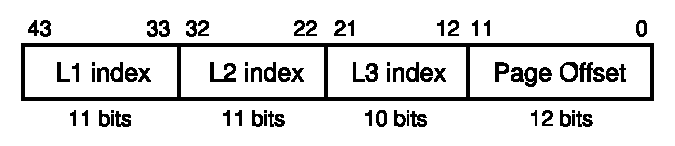
\includegraphics[width=0.45\textwidth]{./gfx/vaddr}
	    \caption{Composición de las direcciones virtuales (4KB).}
	    \label{fig::vaddr4k}
	    \end{figure}

	    Definiendo el overhead de traducción (PTO), como el cociente
	    entre (numerador) la cantidad de memoria fí­sica usada para
	    almacenar las tablas de paginación, y (denominador) la cantidad
	    de memoria fí­sica dedicada a páginas de código y datos de 
	    usuario, ¿cuál es el menor PTO posible en un esquema jerárquico
	    de tres niveles? ¿Cuál es el mayor valor del PTO? Suponer que
	    existe suficiente memoria fí­sica, como para que no haya swap de
	    páginas a disco; y usar PTEs de 64 bit. Además, a los efectos 
	    del cálculo, considerar que el contenido completo de la página
	    alocada es útil.

    \item	MIPS R10000 usa direcciones fí­sicas de 40 bit. La sección de
	    traducción de la TLB contiene el número de página fí­sica 
	    (\verb|PFN|), un bit \verb|V| para indicar si la entrada es
	    válida, un bit \verb|D| (dirty) para indicar que la página
	    necesita ser procesada debido a que fue modificada, y tres bits
	    de estado.

	    ¿Cuál es el tamaño mí­nimo de la PTE, suponiendo páginas de 4KB?

    \item	MIPS/Linux almacena cada PTE en una palabra de 64 bit. Usando
	    la respuesta a la última pregunta, ¿cuántos bits serán
	    desperdiciados?

    \item	\label{asdf}

	    El siguiente comentario, extraí­do de una versión de Linux/MIPS,
	    describe la jerarquía de tres niveles:

	    \begin{verbatim}
		/*
		  * Each address space has 2 4K pages as its page directory, giving
		  * 1024 8 byte pointers to pmd tables. Each pmd table is a pair of
		  * 4K pages, giving 1024 8 byte pointers to page tables. Each (3rd
		  * level) page table is a single 4K page, giving 512 8 byte ptes.
		  */
	    \end{verbatim}

	    Completar el cuadro \ref{tbl::answer}, suponiendo páginas de
	    4KB.

	    \begin{table}
	    \begin{center}
	    \begin{tabular}{|l|l|}
	    \hline
	    \textbf{Index} & \textbf{Longitud en bits}\\ \hline
	    Top-level      & \,                       \\ \hline
	    $2^{nd}$-level & \,                       \\ \hline
	    $3^{rd}$-level & \,                       \\ \hline
	    \end{tabular}
	    \caption{ver ejercicio \ref{asdf}.}
	    \label{tbl::answer}
	    \end{center}
	    \end{table}

    \item	Durante el diseño de un cache 4-way set associative, Raúl R.
	    nota que el cache sufrirá un problema de aliasing homónimo:
	    tal problema sucede cuando dos procesos usan la misma dirección
	    virtual para acceder a lugares fí­sicos distintos.

	    Raúl entonces consulta con el licenciado Varela, quien sugiere
	    agregar un campo PID (process id) al tag virtual. ¿Solucionará
	    esto el problema de aliasing?

	    Otro problema que surge al usar caches virtualmente indexados,
	    y virtualmente taggeados, es la aparición de sinónimos: los
	    mismos aparecen cuando direcciones virtuales distintas refieren
	    al mismo lugar fí­sico. ¿Solucionará este problema la idea del
	    licenciado?

	    Raúl piensa que otra forma de solucionar estos problemas, será
	    usando un cache direct mapped, en vez de set associative. 
	    ¿Tiene razón?
    \end{enumerate}


\subsection{}

  Considerar una máquina con direcciones virtuales de 64 bits y páginas de 4KB.
  Cuenta con una tabla de páginas jerárquica de tres niveles, donde los
  í­ndices L1, L2 y L3 son de 12 bits cada uno. Los bits más significativos
  no se utilizan. Ver cuadro \ref{tbl:vm_addr_fmt}.

  \begin{table}[h]
  \begin{center}
  \begin{tabular}{|c|c|c|c|c|}
  \hline
  unused & L1 index & L2 index & L3 index & page offset \\
  \hline
  \multicolumn{3}{l}{63} & \multicolumn{2}{r}{0} \\
  \end{tabular}
  \caption{Formato de las direcciones virtuales}
  \label{tbl:vm_addr_fmt}
  \end{center}
  \end{table}

  \begin{enumerate}
  \item ¿Cuántas entradas hay en la tabla de páginas del nivel 1?
  \item ¿Cuál es el tamaño de la parte implementada del espacio de direcciones virtuales?
  \item La figura \ref{fig:vm_mem_dump} muestra fragmentos del contenido de la
	tabla de páginas jerárquica de tres niveles (la columna a la izquierda
	corresponde a las direcciones fí­sicas de cada entrada en memoria).

	Las PTEs en las tablas de nivel 1 y 2 contienen la dirección fí­sica
	(PA) a o el número de bloque de disco (DBN) de la tabla del
	siguiente nivel.

	Las PTEs de la tabla de nivel 3 contiene el número de página fí­sica
	(PPN) o el número de bloque de disco (DBN) de la página accedida.
	Las direcciones fí­sicas son de 28 bits.
	
	El tamaño de las PTEs es de 4 bytes, y la dirección base (valor de 
	root pointer) de la tabla actual es 0x0004000. Las direcciones más
	bajas corresponden a los í­ndices más bajos de las tablas de páginas.
	Sólo se muestran las páginas válidas. La columna ``R'' indica el bit
	de página ``residente'' (o presente en memoria).
  
	Para cada dirección virtual dada a continuación, indicar la
	respuesta correcta y llenar el espacio en blanco si corresponde:
  
	\begin{enumerate}
	\item Recorrido de las tablas de paginación para la $VA = 0x0000004010110804$
	      \begin{enumerate}
	      \item Page table entry invalid exception
	      \item Page fault on page table entry
	      \item Page fault, disk block number \underline{$\qquad\qquad\qquad$}
	      \item Redisent, physical address \underline{$\qquad\qquad\qquad$}
	      \end{enumerate}
	\item Recorrido de las tablas de paginación para la $VA = 0x00000001113B0110$
	      \begin{enumerate}
	      \item Page table entry invalid exception
	      \item Page fault on page table entry
	      \item Page fault, disk block number \underline{$\qquad\qquad\qquad$}
	      \item Redisent, physical address \underline{$\qquad\qquad\qquad$}
	      \end{enumerate}
	\item Recorrido de las tablas de paginación para la $VA = 0x0000001101002CD0$
	      \begin{enumerate}
	      \item Page table entry invalid exception
	      \item Page fault on page table entry
	      \item Page fault, disk block number \underline{$\qquad\qquad\qquad$}
	      \item Redisent, physical address \underline{$\qquad\qquad\qquad$}
	      \end{enumerate}
	\end{enumerate}
\begin{figure}[h]
	\centering
	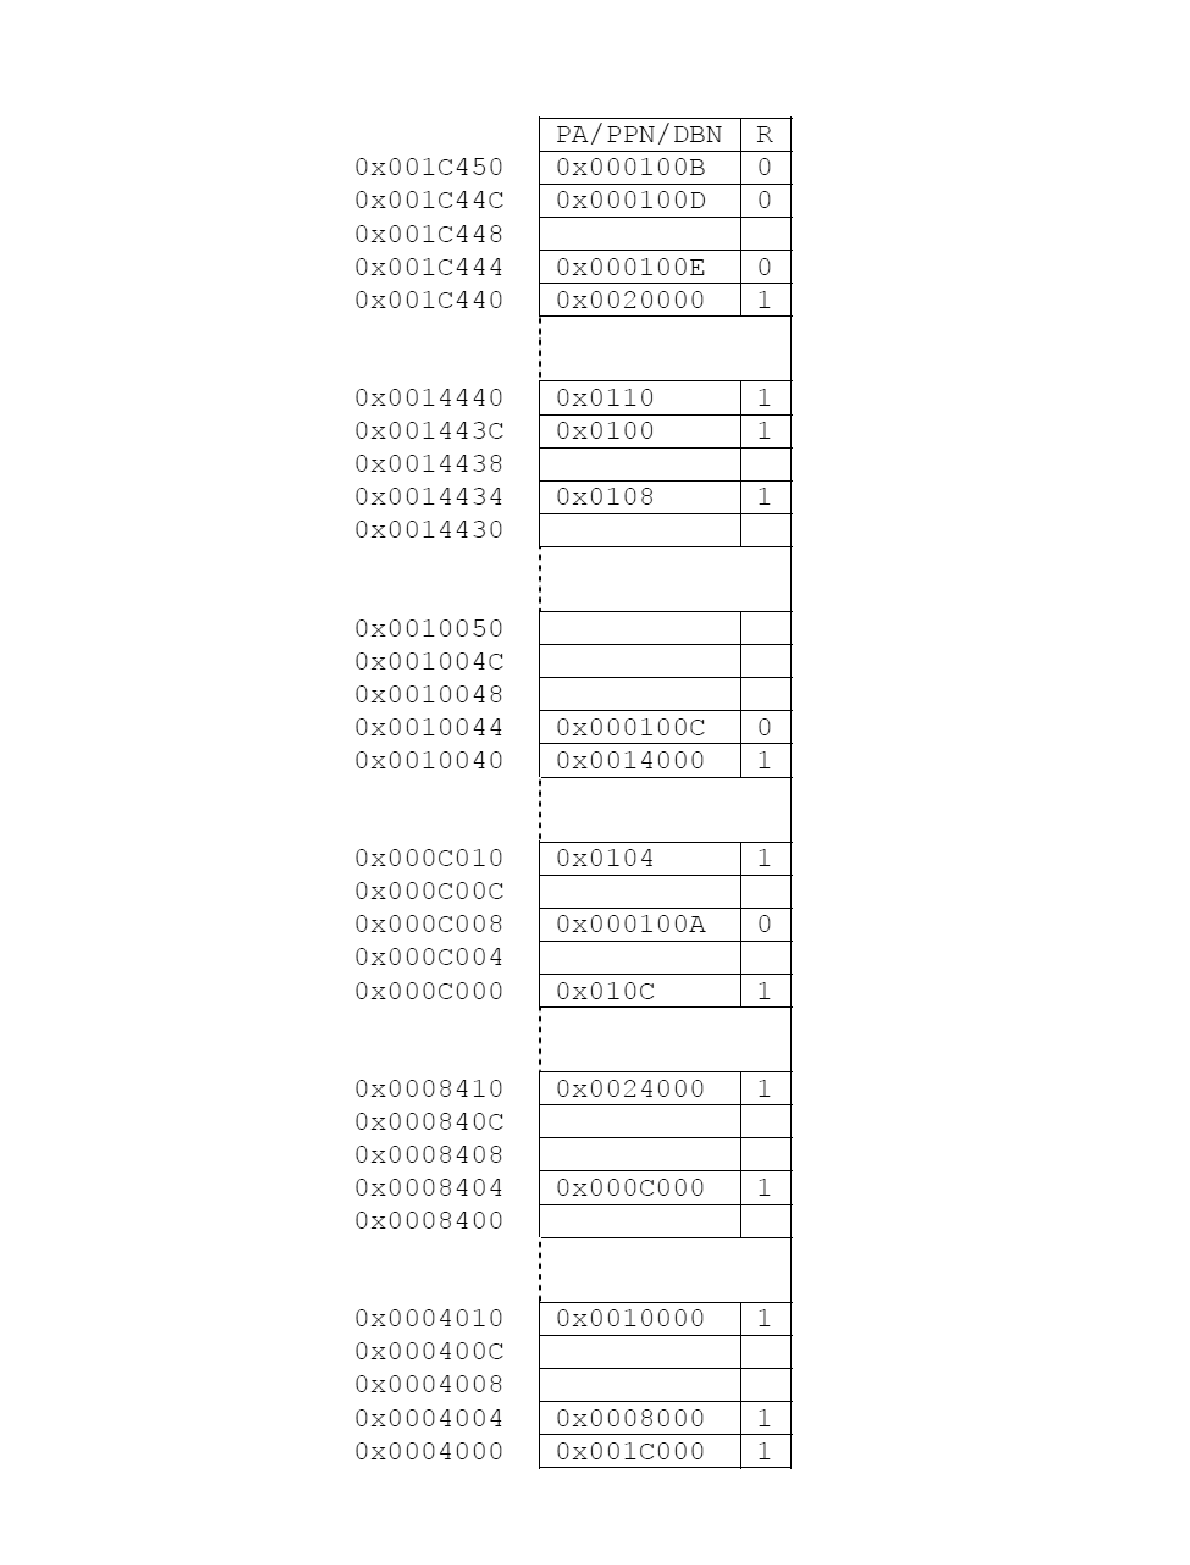
\includegraphics[width=0.7\textwidth]{./gfx/vm_mem_dump}
	\caption{Volcado de memoria en la región de la tabla de páginas}
	\label{fig:vm_mem_dump}
	\end{figure}

	\item La máquina descripta cuenta con un caché
	      único L1, el cual es accedido en paralelo con una TLB fully-associative
	      de 64 entradas. El caché es Direct Mapped, de 16KB, bloques de 4 words,
	      virtually-indexed y physically-tagged. El tamaño del word es de 4 bytes.
	      
	      \begin{enumerate}
	      \item ¿Cuáles de los 64 bits de la dirección virtual son traducidos 
		    por la TLB?
		    \underline{$\qquad\qquad$} : \underline{$\qquad\qquad$}
	      	      
	      \item ¿Cuáles de los 64 bits de la dirección virtual se utilizan para
		    indexar dentro del cache L1?
		    \underline{$\qquad\qquad$} : \underline{$\qquad\qquad$}
	      
	      \item ¿Cuáles de los 28 bits de la dirección fí­sica forman el cache tag?
		    \underline{$\qquad\qquad$} : \underline{$\qquad\qquad$}
	      	      
	      \end{enumerate}
	
	\item En este sistema se previene \emph{aliasing} de la
	      siguiente manera: si dos direcciones virtuales mapean a la misma
	      dirección fí­sica, se requiere que el sistema operativo haga que los
	      page offsets de las direcciones virtuales coincidan. ¿Esto funciona?
	      (justifique, de lo contrario la respuesta se considera automáticamente
	      incorrecta)
	
	\end{enumerate}

\subsection{}
    Sea un sistema de memoria virtual que permite alojar páginas de
    4KB y 4MB. El sistema usa 44 bits efectivos para describir direcciones
    virtuales, y 40 para direcciones físicas. Las páginas de 4KB son
    organizadas usando una tabla jerárquica de tres niveles; y las de 4MB
    se organizan usando los dos primeros niveles de la misma tabla.

    Para distinguir entre ambos casos, las L2 PTEs contienen información
    que indican si el puntero apunta a una tabla L3, o a una página de 4MB.
    Todas las PTEs son de 8 bytes. Ver figura \ref{fig::hier}.

    \begin{figure}[!ht]
    \centering
    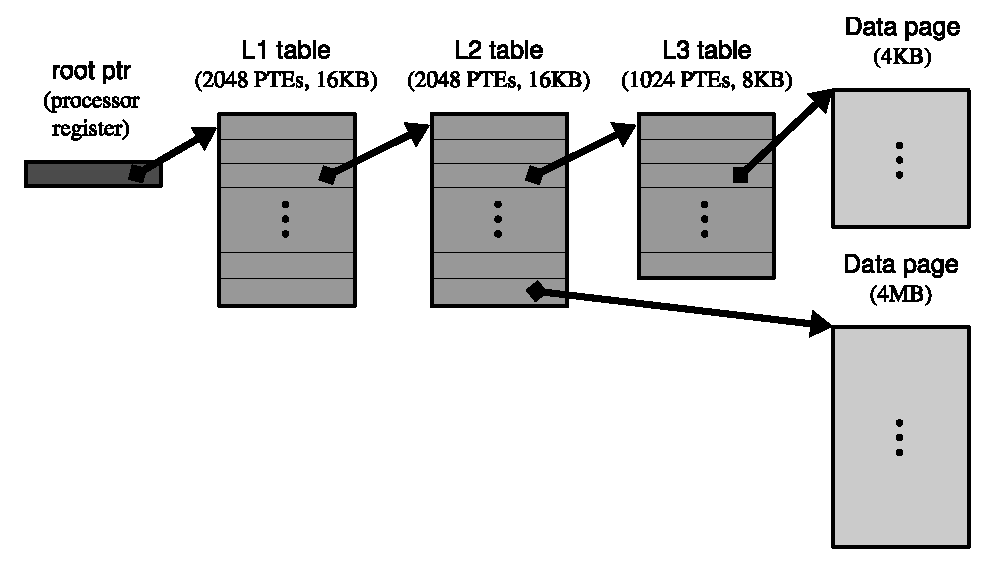
\includegraphics[width=0.6\textwidth]{./gfx/ptes.eps}
    \caption{jerarquía de traducción de direcciones.}
    \label{fig::hier}
    \end{figure}

    El procesador dispone de un TLB de datos con 64 entradas, y cada 
    entrada puede mapearse a cualquiera de los dos tipos de página, 4KB ó
    4MB. Al ocurrir un TLB miss, las tablas de traducción son recorridas
    por hardware, a fin de recargar el TLB. La política de reemplazo es
    FIFO.

    En este ejercicio, evaluaremos la ejecución y utilización de memoria
    del siguiente programa; el mismo es usado para sumar dos arreglos, y
    almacenar el resultado en un tercero:

    \begin{small}
    \begin{verbatim}
	uint8_t A[1048576]; /* 1MB array */
	uint8_t B[1048576]; /* 1MB array */
	uint8_t C[1048576]; /* 1MB array */
	for(int i = 0; i < 1048576; ++i)
		C[i] = A[i] + B[i];
    \end{verbatim}
    \end{small}

    Suponemos, además, que los arreglos \verb|A|, \verb|B|, y \verb|C| 
    están ubicados en una región contigua de memoria física. 
    Consideraremos, además, dos mapeos posibles:

    \begin{itemize}
    \item	4KB: los arreglos son mapeados usando 768 páginas de 4KB (es
	    decir, cada arreglo usa 256 páginas);

    \item	4MB: los arreglos son mapeados usando una única página.
    \end{itemize}

    En las preguntas que siguen, suponer que el programa es el único 
    proceso en el sistema, e ignorar cualquier overhead asociado a la
    ejecución de las instrucciones, o con el sistema operativo. Suponer
    que los arreglos están alineados de tal forma, que minimizan el
    número de PTEs involucradas.

    \begin{enumerate}
    \item	El particionado de la dirección virtual, en el caso de 4KB,
	    es: 11 bits (L1 index), 11 bits (L2 index), 10 bits (L3 index),
	    12 bits (page offset). Ver figura \ref{fig::vaddr4k}.

	    \begin{figure}[!ht]
	    \centering
	    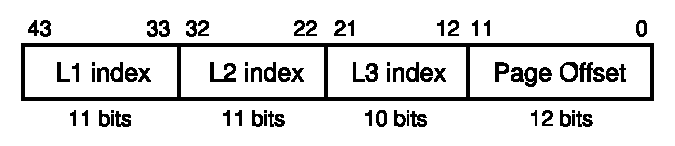
\includegraphics[width=0.45\textwidth]{./gfx/vaddr.eps}
	    \caption{composición de las direcciones virtuales (4KB).}
	    \label{fig::vaddr4k}
	    \end{figure}

	    Mostrar, en forma similar, cómo sería el particionado de una
	    dirección virtual que mapee a una página de 4MB. Incluir el
	    nombre y longitud en bits de todos los campos involucrados.
    
    \item	Definimos el overhead de traducción (PTO), como el cociente 
	    entre (numerador) la cantidad de memoria física usada para
	    almacenar las tablas de paginación, y (denominador) la cantidad
	    de memoria física dedicada a páginas de datos.

	    Para el programa dado anteriormente, ?`cuál es el $PTO_{4KB}$?
	    ?`cuál es el $PTO_{4MB}$?

    \item	Definimos el overhead de fragmentación (PFO), como el cociente
	    entre (numerador) la cantidad de memoria física dedicada a
	    páginas de datos, pero que nunca es accedida; y (denominador)
	    cantidad de memoria física alocada a páginas de datos, 
	    accedida.

	    Para el programa visto, ?`cuánto valen $PFO_{4KB}$ y
	    $PFO_{4MB}$?

    \item	Consideremos ahora la ejecución del programa, suponiendo que
	    la TLB está inicialmente vacía. Para cada uno de los casos
	    (i.e. 4KB y 4MB), ?`cuántos TLB misses ocurren, y cuántos
	    accesos a memoria (PTEs) son necesarios para recargar la TLB?

    \item	?`Cuál de los siguientes números es el mejor candidato para
	    estimar (orden de magnitud) el speedup? 
	    $SU = \left\{1.01; 10; 1000; 1000000\right\}$. Elegir uno, 
	    explicando brevemente tu respuesta. Tomar el caso de 4KB como
	    referencia.
    \end{enumerate}



% \input{./Ejercicios/Memoria2}
% \input{./Ejercicios/Memoria3}
 
\chapter{Pipeline}
El pipelining es una técnica de implementación donde múltiples instrucciones son solapadas en ejecución; toma ventaja del paralelismo que existe entre las acciones requeridas para ejecutar una instrucción.

Un pipeline es como una línea de ensamblado. Por ejemplo, en una línea de ensamblado automotriz, hay muchas etapas, cada una contribuye a la construcción del auto. Cada una opera en paralelo de las otras para diferentes autos. En el pipeline de una computadora, cada etapa completa una parte de la instrucción.

Se define el \textit{throughput} en una línea de ensamblado de autos como el número de autos por hora y se determina por que tan seguido se termina un auto en la línea de montaje. En las computadoras, esto es análogo, y se determina por que tan seguido se completa una instrucción en el pipeline.

Esta técnica de pipelining reduce el tiempo de ejecución promedio por instrucción. Dependiendo de que se considera como base, esta reducción puede ser vista como una reducción en el número de ciclos de reloj por instrucción (CPI) o como una reducción en el tiempo del ciclo de clock o como una combinación. Si se considera un procesador que toma múltiples ciclos de clock por instrucción, entonces pipelining es usualmente visto como una reducción del CPI.




\begin{thebibliography}{9}

    \bibitem{caaqa}
    David Patterson, John Hennessy, \textit{Computer Architecture a Quantitative Approach}, Elsevier, 3rd edition. ISBN: 1-55860-596-7. May 2002.  
  
    \bibitem{coadhsi}

    David Patterson, John Hennessy, \textit{Computer Organization and Design, the Hardware/Software Interface},  Elsevier, 3rd edition. ISBN: 1-55860-604-1. Aug. 2004. 
    
    \bibitem{vmp1}

    B.L. Jacob and T.N. Mudge, \textit{Virtual Memory: Issues of Implementation}, Computer, Vol. 31, No. 6, June 1998, pp. 33-43.

    \bibitem{vmp2}

    B.L. Jacob and T.N. Mudge, \textit{Virtual Memory in Contemporary Microprocessors}, IEEE Micro, Aug. 1998.
    
    \bibitem{mafstocm}

    Jean-Loup Baer, \textit{Microprocessor Architecture. From Simple Pipelines to Chip Multiprocessors}, Cambridge University Press. ISBN-13 978-0-521-76992-1. 2010


    \bibitem{mcch}
    
    Rajeev Balasubramonian and Norman P. Jouppi and Naveen Muralimanohar, \textit{Multi-Core Cache Hierarchies}, Morgan and Claypool Publishers, 2011.
    
    \bibitem{abi}
    
    System V Application Binary Interface, MIPS RISC Processor, 3rd Edition, The Santa Cruz Operation, February 1996 (http://www.sco.com/developers/devspecs/mipsabi.pdf).
\end{thebibliography}
\end{document}
